% =====================================================================
% results.tex — four findings developing one argument about when
% value-directed attention matters:
%   4.1 criterion adjustment typically dominates value encoding
%   4.2-4.3 asymmetry shapes allocation; VDA non-monotonic in r
%   4.4 the graded regime where VDA matters
%   4.5-4.6 no inversion under predictive cues + robustness
% The decorrelation channel rho is reported alongside each finding as a
% sensitivity, per the three-lever decomposition of the Model.
% =====================================================================

\section{Results}
\label{sec:results}

We present four findings that develop a single argument about when
value-directed attention (VDA) matters. First, across the parameter
space the criterion lever \emph{typically} captures the bulk of the
value-related reward gain, as a central tendency with a genuine tail
toward attention-dominated outcomes
(Section~\ref{sec:results-criterion}). Second, the residual VDA benefit
is \emph{non-monotonic} in the benefit/cost ratio $\Rsens$, rising out
of zero, peaking, and decaying again, with a closed-form escape
threshold marking the lower edge of the active band. Third, the
region of $(\valid, \val, \Rsens)$ space in which VDA is materially
large is concentrated, with a \emph{graded} boundary that we map as a
contour band. Fourth, optimal attention does not invert under a
predictive cue --- a \emph{conditional} theorem
(condition $\valid \ge 1/\Nloc$), with inversion in the anti-cue corner
$\valid < 1/\Nloc$ as a new falsifiable prediction. Throughout,
the decorrelation channel $\corr$ (Section~\ref{sec:model}) is reported
\emph{alongside} each finding as a sensitivity: this is the operational
content of the three-lever decomposition
(Definition~\ref{def:three-levers}).

% ---------------------------------------------------------------------
\subsection{Criterion adjustment typically dominates value encoding}
\label{sec:results-criterion}

The first finding concerns how the optimal observer divides the
value-related reward gain between the two adaptive levers available at
fixed correlation: re-aiming the per-location decision criterion (the
criterion shift, $\Rpthree \to \Rpfour$) and re-allocating perceptual
sensitivity (VDA, $\Rpone \to \Rptwo$). The criterion fraction $\CF$
(Eq.~\ref{eq:cf-def}) is the share of the total value-related gain
captured by the criterion lever alone. Across the primary $4{,}410$-cell
$(\Rsens, \valid, \val)$ sweep the criterion lever \emph{typically}
dominates value encoding --- but as a distribution with a central
tendency near three-quarters and a substantial tail, rather than a
uniform bound.

\paragraph{The criterion fraction is a distribution.}
Evaluating the model at the headline configuration
$(\Nloc, \dprimemax, f_0, h) = (4,\,2,\,0.5,\,\sqrt{\;\cdot\;})$ across
the primary sweep ($\valid \in [0.25, 1.00]$, $21$ points;
$\Rsens \in [0.1, 10]$, $22$ values --- $21$ log-spaced plus a pinned
$\Rsens = 1$; $\val \in \{1,2,3,4,5\}$; both reward variants), of whose
$4{,}620$ nominal cells $4{,}410$ ($2{,}205$ per variant) yield valid,
non-degenerate optima, gives the $\CF$
distribution of Table~\ref{tab:cf-distribution}. The median $\CF$ is
$0.7552$ (variant~A) and $0.7682$ (variant~B), well above $0.5$, while
the distribution spans a wide range at both ends. Variant~A's strict
minimum is $0.5587$; variant~B's is $0.3040$, with $8\%$ of variant-B
cells falling under $0.50$. At the upper end both variants reach
$\CF = 1.00$. The finding is therefore a \emph{central-tendency} one:
the criterion lever captures roughly three-quarters of the
value-related reward gain in a typical cell, with a left tail --- much
heavier in variant~B --- in which it captures substantially less.
Figure~\ref{fig:cf-histogram} shows the full per-cell distribution.

\begin{table}[t]
  \centering
  \small
  \begin{tabular}{l c c c c c c c c}
    \toprule
    variant & $\CF_{\min}$ & $q_{5\%}$ & $q_{25\%}$ & median &
    $q_{75\%}$ & $q_{95\%}$ & $\CF_{\max}$ & mean $\pm$ s.d.\\
    \midrule
    A & $0.5587$ & $0.5931$ & $0.6530$ & $\mathbf{0.7552}$
      & $0.8996$ & $1.0000$ & $1.0000$
      & $0.7773 \pm 0.1363$\\
    B & $\mathbf{0.3040}$ & $0.4564$ & $0.6288$ & $\mathbf{0.7682}$
      & $0.9463$ & $1.0000$ & $1.0000$
      & $0.7691 \pm 0.1808$\\
    \bottomrule
  \end{tabular}
  \caption{Distribution of the criterion fraction $\CF$
  (Eq.~\ref{eq:cf-def}) across the primary $4{,}410$-cell
  $(\Rsens, \valid, \val)$ sweep at the headline configuration
  $(\Nloc, \dprimemax, f_0, h) = (4,\,2,\,0.5,\,\sqrt{\;\cdot\;})$ under
  independence $\corr = 0$, per reward variant. Quantiles are over
  the $n = 2{,}205$ valid cells per variant. The median (boldface) sits
  near three-quarters in both variants, with a wide spread toward lower
  $\CF$.}
  \label{tab:cf-distribution}
\end{table}

\begin{figure}[t]
  \centering
  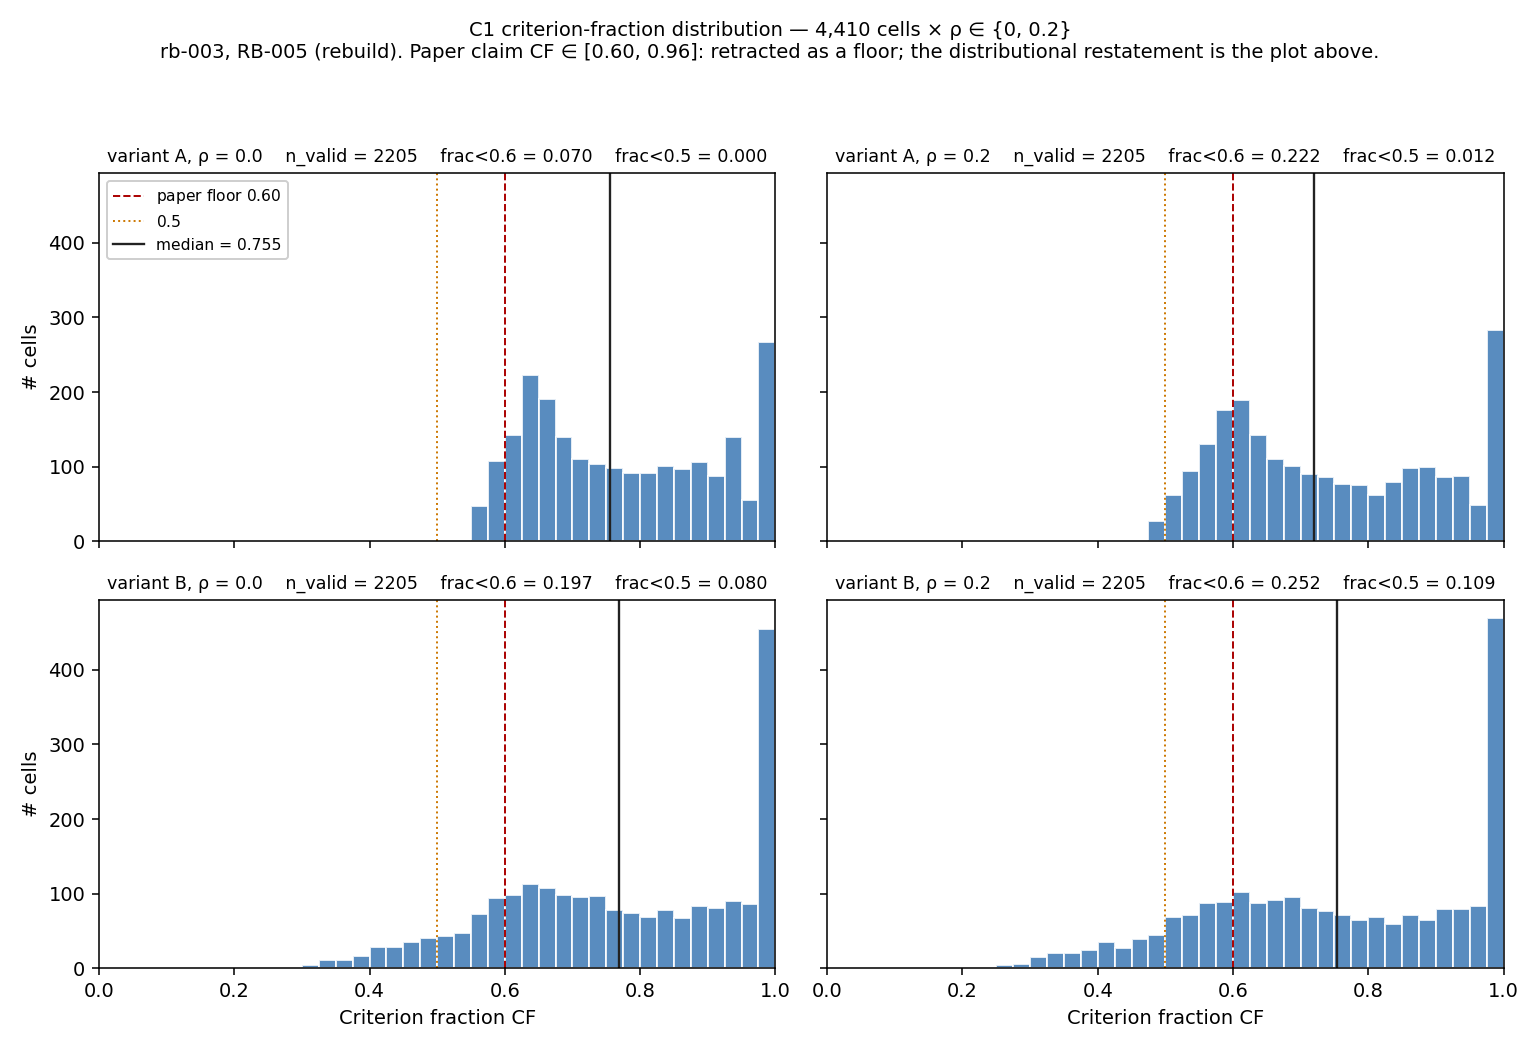
\includegraphics[width=0.92\linewidth]{figures/cf_histogram.png}
  \caption{Per-cell histogram of the criterion fraction $\CF$ across the
  $4{,}410$-cell sweep (columns: reward variant; rows:
  decorrelation $\corr \in \{0, 0.2\}$). The distribution --- a broad
  mode near $\CF \approx 0.65$, a left tail (much heavier in variant~B),
  and a spike at $\CF = 1$ --- characterises how the criterion fraction
  is spread across the parameter space. The $\corr = 0.2$ row exhibits
  the decorrelation amplification of the left tail quantified below.}
  \label{fig:cf-histogram}
\end{figure}

\paragraph{Where the criterion lever dominates, and where it cedes.}
The marginal distribution obscures the \emph{regime} structure that
drives it. Partitioning the cells by benefit/cost regime
($\Rsens < 1$ cost-dominant, $\Rsens = 1$ symmetric, $\Rsens > 1$
benefit-dominant) and validity ($\valid < 1/2$ vs.\ $\valid \ge 1/2$)
exposes a clean ordering (Table~\ref{tab:cf-quadrants}): $\CF$ decreases
monotonically along the $\Rsens$ axis from the cost-dominant corner
(median $\CF \ge 0.90$ in both variants --- criterion captures almost
everything) to the benefit-dominant, low-validity corner, where it
cedes the lead to attention re-allocation (variant~A median $0.61$ with
$37\%$ of cells below $0.6$; variant~B median $0.51$ with $78\%$ below
$0.6$ and a strict minimum of $0.30$). Read off the quadrant medians,
the ordering runs from $\CF$ near unity in the cost-dominant regime,
through roughly three-quarters at symmetry, to a benefit-dominant,
low-validity corner in which the criterion lever is no longer dominant.
Figure~\ref{fig:cf-heatmap} displays the same structure cell-wise over
the $(\Rsens, \valid)$ plane, and Figure~\ref{fig:cf-curves} shows
$\CF(\Rsens)$ declining from near unity as the benefit/cost ratio rises.
The criterion lever thus tends to unity at small $\Rsens$ and declines
at large $\Rsens$, with the share it captures spread over a wide range
across the parameter space.

\begin{table}[t]
  \centering
  \small
  \begin{tabular}{l l r r r r}
    \toprule
    variant & $\Rsens$-regime ($\valid$) &
    median $\CF$ & strict min &
    $\mathrm{frac}\!<\!0.6$ & $n$\\
    \midrule
    A & cost-dom., $\valid$ low     & $0.998$ & $0.825$ & $0.000$ & $350$\\
    A & cost-dom., $\valid$ high    & $0.897$ & $0.825$ & $0.000$ & $385$\\
    A & symmetric, $\valid$ low     & $0.779$ & $0.665$ & $0.000$ & $350$\\
    A & symmetric, $\valid$ high    & $0.740$ & $0.665$ & $0.000$ & $385$\\
    A & benefit-dom., $\valid$ high & $0.645$ & $0.563$ & $0.062$ & $385$\\
    A & benefit-dom., $\valid$ low  & $\mathbf{0.612}$ & $\mathbf{0.559}$
                                    & $\mathbf{0.374}$ & $350$\\
    \midrule
    B & cost-dom., $\valid$ low     & $1.000$ & $0.905$ & $0.000$ & $350$\\
    B & cost-dom., $\valid$ high    & $0.931$ & $0.797$ & $0.000$ & $385$\\
    B & symmetric, $\valid$ low     & $0.800$ & $0.497$ & $0.103$ & $350$\\
    B & symmetric, $\valid$ high    & $0.753$ & $0.575$ & $0.010$ & $385$\\
    B & benefit-dom., $\valid$ high & $0.630$ & $0.469$ & $0.317$ & $385$\\
    B & benefit-dom., $\valid$ low  & $\mathbf{0.509}$ & $\mathbf{0.304}$
                                    & $\mathbf{0.780}$ & $350$\\
    \bottomrule
  \end{tabular}
  \caption{Quadrant breakdown of $\CF$ at $\corr = 0$. The criterion
  lever dominates uniformly in the cost-dominant region (median
  $\CF \ge 0.90$ in both variants) and cedes to attention re-allocation
  in the benefit-dominant, low-validity corner, where its median falls
  to $0.61$ (variant~A) and $0.51$ (variant~B).}
  \label{tab:cf-quadrants}
\end{table}

\begin{figure}[t]
  \centering
  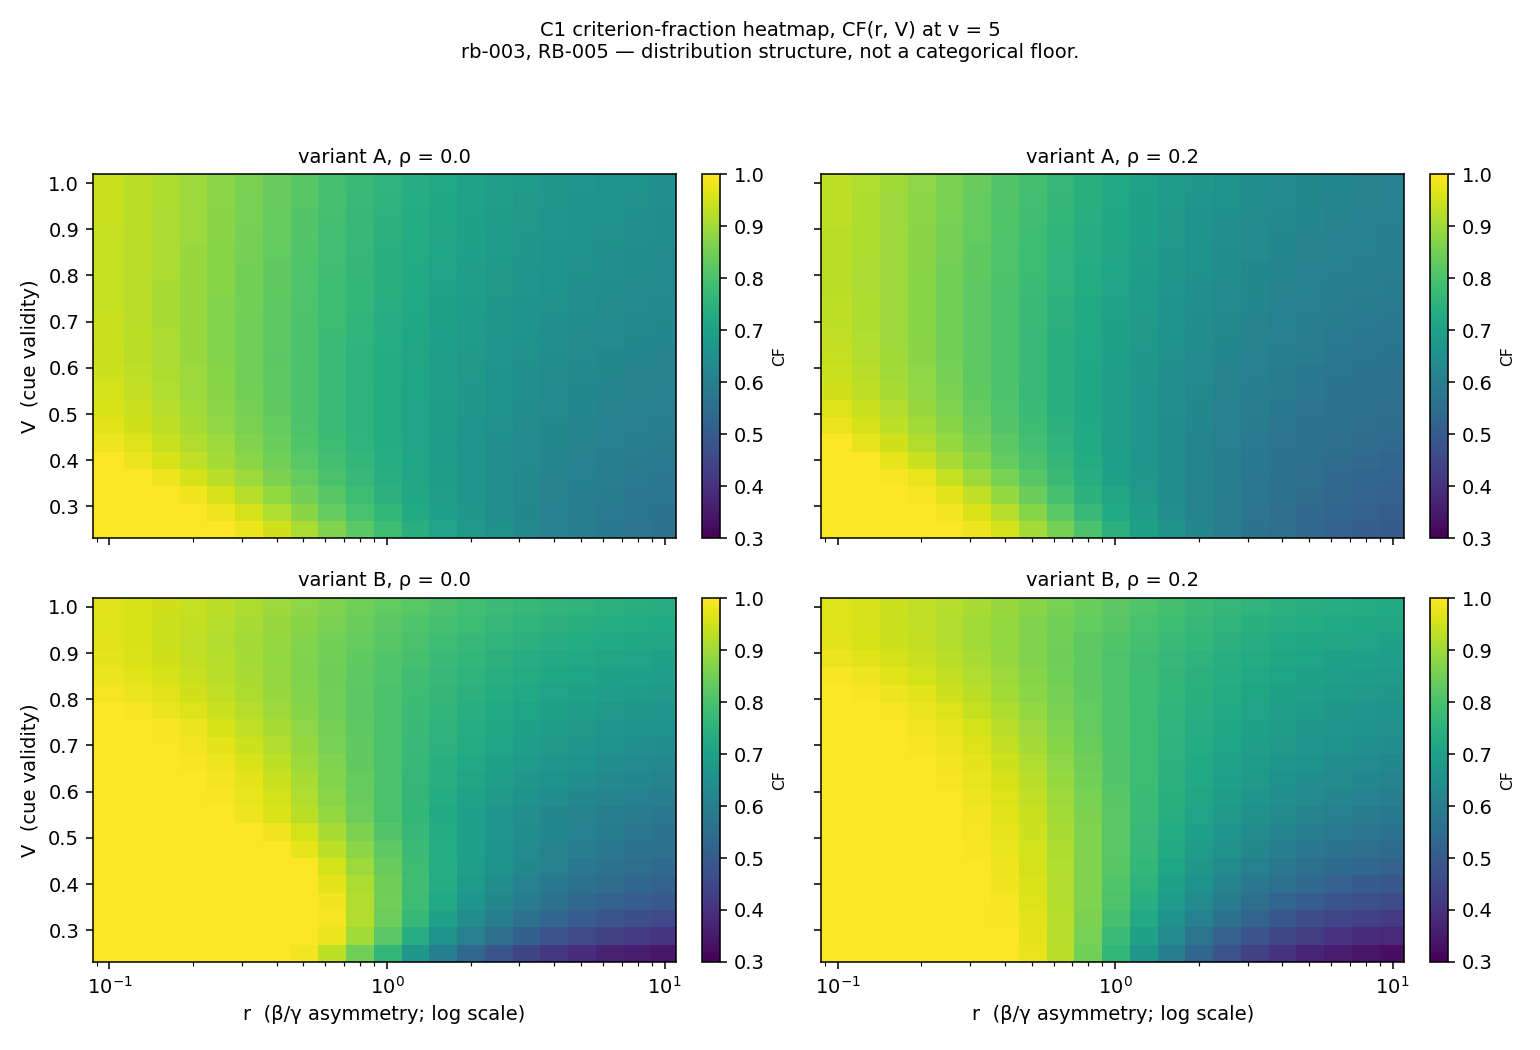
\includegraphics[width=0.92\linewidth]{figures/cf_heatmap.png}
  \caption{$\CF$ over the $(\Rsens, \valid)$ plane at $\val = 5$,
  $(\Nloc, \dprimemax, f_0, h) = (4,\,2,\,0.5,\,\sqrt{\;\cdot\;})$
  (rows: $\corr$; columns: variant). The diagonal boundary in
  $(\log \Rsens, \valid)$ separates the criterion-dominated region
  ($\CF$ near $1$, low $\Rsens$) from the attention-dominated corner
  ($\CF$ low, high $\Rsens$, low $\valid$) of
  Table~\ref{tab:cf-quadrants}. The low-$\CF$ corner is wider in
  variant~B and widens further at $\corr = 0.2$.}
  \label{fig:cf-heatmap}
\end{figure}

\begin{figure}[t]
  \centering
  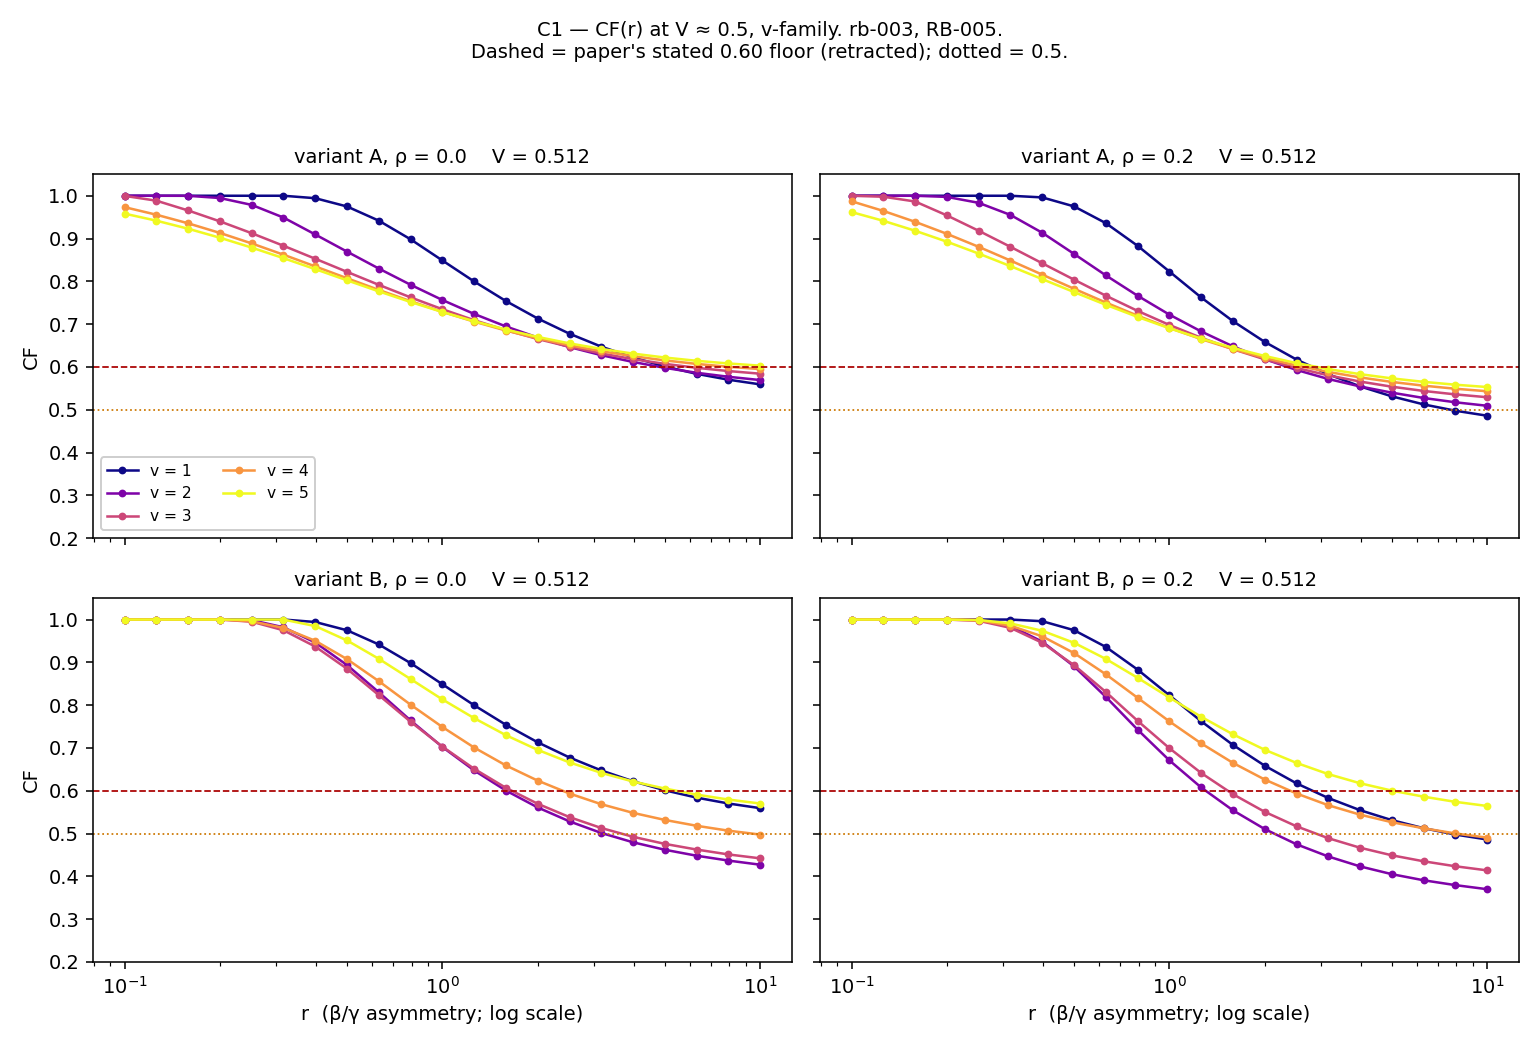
\includegraphics[width=0.92\linewidth]{figures/cf_curves.png}
  \caption{$\CF(\Rsens)$ at $\valid \approx 0.5$ as a $\val$-family
  $\val \in \{1,2,3,4,5\}$ (rows: $\corr$; columns: variant). At small
  $\Rsens$ (cost-dominant) the curves cluster near $\CF = 1$; as
  $\Rsens$ increases they decline, more steeply for larger $\val$,
  exposing the benefit-dominant region in which attention re-allocation
  overtakes the criterion shift.}
  \label{fig:cf-curves}
\end{figure}

\paragraph{Decorrelation sensitivity.}
Admitting correlated noise reshapes the criterion fraction in a
variant-specific way. Running the full sweep at $\corr = 0.2$ --- the
cross-location correlation magnitude reported for visual cortex
\cite{CohenMaunsell2009} --- the criterion fraction falls in variant~A.
Raising $\corr$ from $0$ to $0.2$ amplifies the variant-A left tail by
roughly a factor of three (the fraction of cells with $\CF < 0.6$ rises
from $0.07$ to $0.22$) and pushes the strict minimum below $0.50$;
cell-wise, $\CF$ decreases in $84\%$ of variant-A cells (median
$\Delta\CF = -0.035$). In variant~B the response is mixed: $64\%$ of
cells decrease while $24\%$ increase, consistent with an essentially
flat variant-B sensitivity. The decorrelation channel thus reduces
$\CF$ on a typical variant-A cell and leaves it essentially unchanged,
with substantial scatter, on a typical variant-B cell. The sign of
$\partial\VDA/\partial\corr$ is itself non-uniform and is taken up with
the VDA findings below and in the Discussion
(Section~\ref{sec:discussion}).

\paragraph{Robustness to the conservation rule.}
The benefit and cost weights $(\benefit, \cost)$ satisfy a conservation
constraint (Section~\ref{sec:model}); the numbers above are reported at
its additive endpoint ($\benefit + \cost = 2$), one member of a
one-parameter family whose opposite endpoint is multiplicative
($\benefit \cdot \cost = 1$). Sweeping that family at each reward variant,
the central tendency of $\CF$ is robust while the tail is not. Moving from the additive to the multiplicative endpoint leaves the
median essentially fixed (variant~A $-0.0012$; variant~B $-0.0042$) but
roughly doubles the fraction of cells with $\CF < 0.5$ (from $4.0\%$ to
$8.3\%$, combined), drives $191$ cells from $\CF \ge 0.5$ to $\CF < 0.5$
with no cell moving the other way, and deepens the variant-B minimum
from $0.304$ to $0.231$. The conservation-family treatment of these band
endpoints is given in the Discussion (Section~\ref{sec:discussion}); for
the present finding the conclusion is that the ``criterion typically
dominates'' central tendency is invariant to the conservation rule,
whereas the size of the tail in which it does not dominate is
rule-dependent.

% ---------------------------------------------------------------------
\subsection{The value-directed attention benefit is non-monotonic in
            the benefit/cost ratio}
\label{sec:results-vda-nonmonotonic}

The first finding fixed the cross-location correlation and asked how the
optimal observer splits the value-related gain between the criterion and
attention levers. We now follow the attention lever itself across the
benefit/cost ratio $\Rsens$ and find that its contribution is
\emph{non-monotonic}: the value-directed attention benefit
$\VDA(\Rsens) = \Rpone(\Rsens) - \Rptwo(\Rsens)$
(Eq.~\ref{eq:vda-def}) rises out of zero at small $\Rsens$, reaches an
interior maximum, and decays back toward zero as $\Rsens \to \infty$.
This shape is the model's signature: attention re-allocation pays off
only in an intermediate band of the benefit/cost ratio, and the model
delivers a closed-form expression for the lower edge of that band.

\paragraph{A closed-form escape threshold.}
The asymmetry between the reward for a benefit (correctly attending the
high-value cued location) and the cost (a miss or a false alarm) governs
when re-allocating sensitivity away from uniform attention first becomes
worthwhile. Differentiating the joint-optimum expected reward
$\Rpone(\alpha, \Rsens)$ with respect to the cued-attention share
$\alpha$ and evaluating at the uniform allocation $\alpha = 1/\Nloc$,
the first-order condition $\partial_\alpha \Rpone|_{1/\Nloc} = 0$
defines the value of the benefit/cost ratio at which the optimiser
begins to move attention toward the cued location. Writing
$\dprime_b \equiv \dprime_{\mathrm{base}} = \dprimemax\, f(1/\Nloc)$ for
the baseline discriminability under uniform attention
(Section~\ref{sec:model}) and $(c_c^\star, c_u^\star)$ for the
per-location optimal criterion pair at $\alpha = 1/\Nloc$, this escape
threshold is
%
\begin{equation}
  \rdagger(\val) \;=\; \frac{K_u(\val)}{(\Nloc - 1) \cdot K_c(\val)},
  \label{eq:r-dagger}
\end{equation}
%
with per-location gradient coefficients
%
\begin{align}
  K_c(\val) &= \tfrac{1}{4}\Big[
    \valid\, \val\, \varphi\!\big(\tfrac{\dprime_b}{2} - c_c^\star\big)
    \;+\; \CR(\val)\, \varphi\!\big(\tfrac{\dprime_b}{2} + c_c^\star\big)\,
    \Phinorm\!\big(\tfrac{\dprime_b}{2} + c_u^\star\big)^{\Nloc - 1}
  \Big],
  \label{eq:K-c}
  \\[2pt]
  K_u(\val) &= \tfrac{1}{4}\Big[
    (1 - \valid)\, \varphi\!\big(\tfrac{\dprime_b}{2} - c_u^\star\big)
    \;+\; (\Nloc - 1)\, \CR(\val)\, \Phinorm\!\big(\tfrac{\dprime_b}{2}
    + c_c^\star\big)
    \notag\\
    &\qquad\quad\;\;\;\;\;\;\;\;\;\;\;\;\;\;\;\;\;\;\;\;\;\;\;
    \cdot\, \Phinorm\!\big(\tfrac{\dprime_b}{2} + c_u^\star\big)^{\Nloc - 2}
    \varphi\!\big(\tfrac{\dprime_b}{2} + c_u^\star\big)
  \Big].
  \label{eq:K-u}
\end{align}
%
The factor $\CR(\val)$ is the correct-rejection reward scaling set by
the reward variant (Section~\ref{sec:model}); the value-blind reference
used throughout this section takes $\CR(\val) = 1$, with the benefit and
cost weights following the additive conservation rule
($\benefit + \cost = 2$). The threshold
\eqref{eq:r-dagger} is a consequence of the model definitions rather
than an empirical regularity; its derivation is given in the
Supplementary material (Section~\ref{sec:appendix}).

\paragraph{The threshold falls as cued value rises.}
Evaluating Eqs.~\eqref{eq:r-dagger}--\eqref{eq:K-u} at the configuration
$(\Nloc, \dprimemax, f_0, h, \valid) = (4,\,2,\,0.5,\,\sqrt{\;\cdot\;},\,0.5)$
gives the values in
Table~\ref{tab:r-dagger-family}. The escape threshold decreases
monotonically in the cued value $\val$, from $\rdagger \approx 0.34$ at
$\val = 1$ to $\rdagger \approx 0.02$ at $\val = 10$: the more reward a
correct cued response carries, the smaller the benefit/cost asymmetry
needed before attention re-allocation begins to pay. Figure~\ref{fig:r-dagger-vs-v}
plots $\rdagger(\val)$ as a continuous curve with these family points
marked.

\begin{table}[t]
  \centering
  \small
  \begin{tabular}{r r r r r r}
    \toprule
    $\val$ &
    $\rdagger(\val)$ &
    $c_c^\star$ &
    $c_u^\star$ &
    $K_c(\val)$ &
    $K_u(\val)$ \\
    \midrule
    $1$  & $0.343$ & $\phantom{-}0.40$ & $1.05$ & $0.0930$ & $0.0958$ \\
    $2$  & $0.168$ & $\phantom{-}0.25$ & $1.30$ & $0.1734$ & $0.0872$ \\
    $3$  & $0.099$ & $\phantom{-}0.15$ & $1.50$ & $0.2532$ & $0.0755$ \\
    $5$  & $0.050$ & $\phantom{-}0.10$ & $1.75$ & $0.4065$ & $0.0615$ \\
    $8$  & $0.022$ & $\phantom{-}0.05$ & $2.05$ & $0.6357$ & $0.0424$ \\
    $10$ & $0.016$ & $\phantom{-}0.05$ & $2.15$ & $0.7864$ & $0.0380$ \\
    \bottomrule
  \end{tabular}
  \caption{Closed-form escape threshold $\rdagger(\val) = K_u(\val) /
  [(\Nloc - 1)\,K_c(\val)]$ from \eqref{eq:r-dagger}--\eqref{eq:K-u} at
  $(\Nloc, \dprimemax, f_0, h, \valid) = (4,\,2,\,0.5,\,\sqrt{\;\cdot\;},\,0.5)$,
  additive conservation. The $\val = 1$ row is the symmetric reference
  $\rdagger(1) \approx 0.343$; the threshold falls monotonically as the
  cued value grows.}
  \label{tab:r-dagger-family}
\end{table}

\begin{figure}[t]
  \centering
  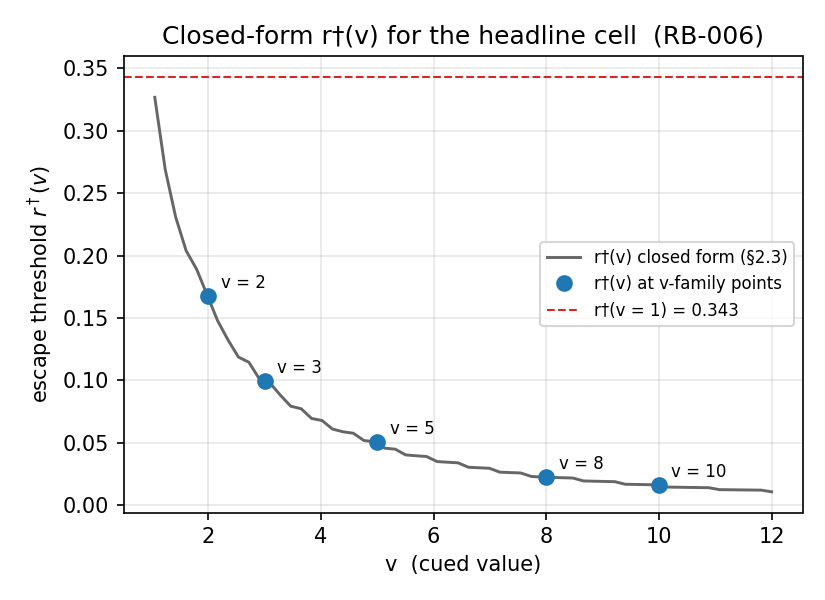
\includegraphics[width=0.7\linewidth]{figures/r_dagger_vs_v.png}
  \caption{The closed-form escape threshold $\rdagger(\val)$ at
  $(\Nloc, \dprimemax, f_0, h, \valid) = (4,\,2,\,0.5,\,\sqrt{\;\cdot\;},\,0.5)$,
  additive conservation. The continuous curve is computed from
  \eqref{eq:r-dagger}--\eqref{eq:K-u} on a dense $\val$-grid, with the
  family points $\val \in \{2,3,5,8,10\}$ marked. The horizontal
  reference $\rdagger(1) \approx 0.343$ is the symmetric upper anchor of
  the family. The threshold marks the benefit/cost ratio at which the
  optimal observer first leaves uniform attention.}
  \label{fig:r-dagger-vs-v}
\end{figure}

\paragraph{The peak benefit sits inside the predicted band.}
The escape threshold marks where the joint optimum P1 \emph{begins} to
depart from uniform attention. The value-blind baseline P2, against
which VDA is measured, leaves uniform attention only at the higher
threshold $\rdagger(\val{=}1)$ --- the symmetric reference, because P2
allocates attention as if every location carried equal value. The VDA
benefit therefore opens up on the interior interval
$(\rdagger(\val),\, \rdagger(1))$, where P1 has re-allocated but P2 has
not, and closes again once P2 also escapes uniform attention. This
predicts that the peak of $\VDA(\Rsens)$ lies strictly above
$\rdagger(\val)$. A high-resolution sweep of $84$ points in $\Rsens$
($83$ log-spaced over $[0.1, 10]$ plus pinned escape- and
peak-neighbourhood points) confirms it: the peak $r^\star =
\arg\max_{\Rsens}
\VDA(\Rsens)$ exceeds $\rdagger(\val)$ for every $\val$ in the family,
by a margin of $0.28$ to $0.35$, and clusters just below the symmetric
anchor $\rdagger(1) \approx 0.34$ (Table~\ref{tab:peak-vs-threshold}).

\begin{table}[t]
  \centering
  \small
  \begin{tabular}{r r r r c}
    \toprule
    $\val$ &
    $\rdagger(\val)$ &
    $r^\star$ &
    $r^\star - \rdagger(\val)$ &
    above? \\
    \midrule
    $2$  & $0.168$ & $0.501$ & $+0.334$ & \checkmark \\
    $3$  & $0.099$ & $0.376$ & $+0.276$ & \checkmark \\
    $5$  & $0.050$ & $0.376$ & $+0.325$ & \checkmark \\
    $8$  & $0.022$ & $0.376$ & $+0.354$ & \checkmark \\
    $10$ & $0.016$ & $0.355$ & $+0.339$ & \checkmark \\
    \bottomrule
  \end{tabular}
  \caption{Empirical peak $r^\star = \arg\max_{\Rsens} \VDA(\Rsens)$
  against the closed-form escape threshold $\rdagger(\val)$ at
  $(\Nloc, \dprimemax, f_0, h, \valid) = (4,\,2,\,0.5,\,\sqrt{\;\cdot\;},\,0.5)$,
  $\corr = 0$. The peak lies above $\rdagger(\val)$ for every $\val$ and
  clusters near the symmetric anchor $\rdagger(1) \approx 0.343$,
  consistent with the prediction that $\VDA$ is supported on the
  interval $(\rdagger(\val),\, \rdagger(1))$. Peak located on an
  $84$-point log-grid in $\Rsens$.}
  \label{tab:peak-vs-threshold}
\end{table}

Figure~\ref{fig:vda-curves-vfamily} shows the full $\VDA(\Rsens)$
family. The peak height grows monotonically with cued value, from
$\VDA \approx 0.012$ at $\val = 2$ to $\VDA \approx 0.183$ at
$\val = 10$, and each peak sits above its corresponding threshold
$\rdagger(\val)$ (dashed verticals). The benefit of value-directed
attention is thus largest precisely where the cued location is most
valuable and the benefit/cost asymmetry is moderate --- not at the
extremes of $\Rsens$, where either the criterion lever alone suffices
(small $\Rsens$) or both policies have already re-allocated (large
$\Rsens$).

\begin{figure}[t]
  \centering
  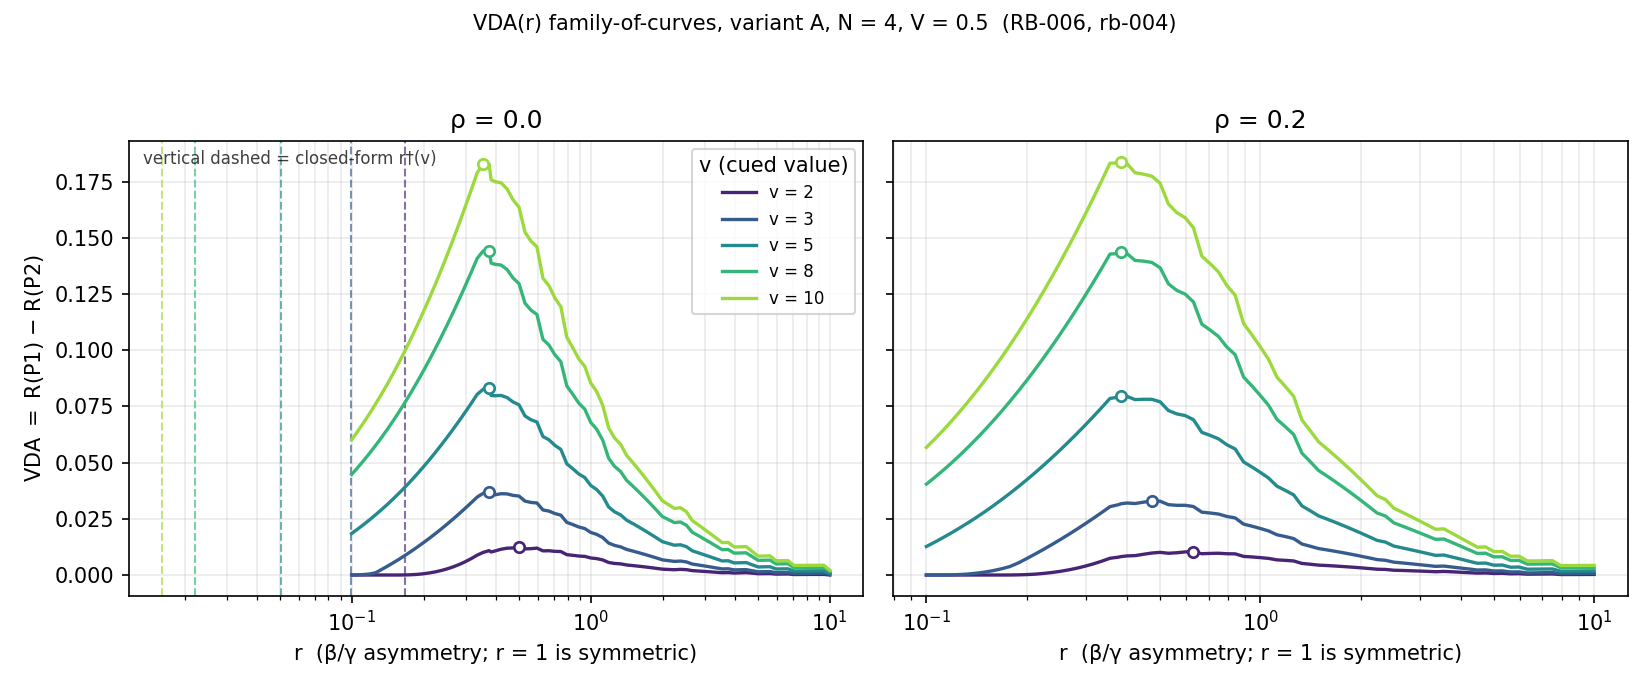
\includegraphics[width=0.95\linewidth]{figures/vda_curves_vfamily.png}
  \caption{Non-monotonicity of $\VDA(\Rsens)$ in the benefit/cost ratio
  across a $\val$-family at
  $(\Nloc, \dprimemax, f_0, h, \valid) = (4, 2, 0.5, \sqrt{\;\cdot\;}, 0.5)$,
  additive conservation. \textbf{Left:} $\corr = 0$. Each curve rises
  from zero, peaks in the interior, and decays; the closed-form escape
  threshold $\rdagger(\val)$ from \eqref{eq:r-dagger} is overlaid as a
  vertical dashed line per $\val$, and the empirical peak (white-filled
  dot) lies above $\rdagger(\val)$ for every $\val$
  (Table~\ref{tab:peak-vs-threshold}). \textbf{Right:} the same family
  at $\corr = 0.2$; correlated noise suppresses the peak at low $\val$
  but amplifies it at $\val = 10$, so the sign of
  $\partial \VDA^\star / \partial \corr$ depends on the cued value
  (Table~\ref{tab:rho-sensitivity}).}
  \label{fig:vda-curves-vfamily}
\end{figure}

\paragraph{Decorrelation sensitivity.}
The sign of the decorrelation lever's effect on the VDA benefit depends
on the cued value, not on the benefit/cost ratio alone. Raising the
cross-location correlation from $\corr = 0$ to $\corr = 0.2$ --- the
magnitude reported for visual cortex \cite{CohenMaunsell2009} --- and
re-measuring the peak benefit across the $\val$-family
(Table~\ref{tab:rho-sensitivity}) \emph{suppresses} the peak for
$\val \le 8$ (by up to $\Delta\VDA^\star = -0.004$ at $\val = 3$) but
\emph{amplifies} it at $\val = 10$ ($\Delta\VDA^\star = +0.001$). The
peak location $r^\star$ also drifts upward in $\corr$, most visibly at
low $\val$, where it rises from $0.501$ to $0.631$ at $\val = 2$. This
upward drift has a closed-form counterpart: extending the threshold
\eqref{eq:r-dagger}--\eqref{eq:K-u} to $\corr > 0$ by replacing the
no-false-alarm terms in $K_c, K_u$ with their correlation-aware
one-dimensional Gauss--Hermite gradients (Section~\ref{sec:appendix})
yields $\rdagger(\val;\corr)$, and predicts
$\rdagger(\val; 0.2) > \rdagger(\val; 0)$ at every $\val$ --- the lower
edge of the active band drifts up by $+3\%$ at $\val = 1$ to $+30\%$ at
$\val = 8$, matching the sign of the empirical peak drift at every
$\val \neq 1$. The decorrelation lever therefore does not uniformly
attenuate the VDA benefit: in the strongly benefit-dominant, high-value
corner it \emph{enhances} the benefit, and across the family it shifts
the active band toward larger $\Rsens$. This is the operational meaning
of treating decorrelation as a third independent lever
(Definition~\ref{def:three-levers}): its effect on attention is
signed by the value structure of the task.

\begin{table}[t]
  \centering
  \small
  \begin{tabular}{r r r r r r}
    \toprule
    $\val$ &
    $\VDA^\star\,(\corr{=}0)$ &
    $\VDA^\star\,(\corr{=}0.2)$ &
    $\Delta \VDA^\star$ &
    $r^\star\,(\corr{=}0)$ &
    $r^\star\,(\corr{=}0.2)$ \\
    \midrule
    $2$  & $0.01233$ & $0.01036$ & $-0.00197$ & $0.501$ & $0.631$ \\
    $3$  & $0.03698$ & $0.03291$ & $-0.00407$ & $0.376$ & $0.473$ \\
    $5$  & $0.08300$ & $0.07954$ & $-0.00345$ & $0.376$ & $0.383$ \\
    $8$  & $0.14422$ & $0.14355$ & $-0.00067$ & $0.376$ & $0.383$ \\
    $10$ & $0.18284$ & $0.18387$ & $\mathbf{+0.00103}$ & $0.355$ & $0.383$ \\
    \bottomrule
  \end{tabular}
  \caption{Decorrelation sensitivity of the peak VDA benefit at
  $(\Nloc, \dprimemax, f_0, h, \valid) = (4, 2, 0.5, \sqrt{\;\cdot\;}, 0.5)$,
  additive conservation. Raising $\corr$ from $0$ to $0.2$ suppresses
  peak $\VDA^\star$ for $\val \le 8$ and amplifies it at $\val = 10$,
  while the peak location $r^\star$ drifts upward (most visibly at low
  $\val$). The sign of $\partial \VDA^\star / \partial \corr$ thus
  depends on the cued value.}
  \label{tab:rho-sensitivity}
\end{table}

\paragraph{Scope.}
The threshold and family numerics above are reported under additive
conservation ($\benefit + \cost = 2$, $\CR(\val) = 1$) at
$\valid = 0.5$; the correlation-aware extension of
\eqref{eq:r-dagger}--\eqref{eq:K-u} and its drift table are developed in
the Supplementary material (Section~\ref{sec:appendix}). The
sensitivity of the peak magnitudes to the conservation rule is taken up
with the conservation-family band in the Discussion
(Section~\ref{sec:discussion}).

% ---------------------------------------------------------------------
% Results: the graded regime where VDA is materially large; iso-VDA
% contour band over (V, v); quantitative high-validity design guidance.
\subsection{The benefit is concentrated in a graded regime}
\label{sec:results-graded}

The non-monotonicity of Section~\ref{sec:results-vda-nonmonotonic}
locates the active band along the $\Rsens$-axis at a fixed design
point. Sweeping the experimental-design plane $(\valid, \val)$ shows
that the value-directed attention benefit is materially large only in a
concentrated corner of the design space --- low cue validity, high
value contrast, and moderate-to-low benefit/cost asymmetry --- and that
this corner has a \emph{graded} boundary. We map the boundary as an
iso-VDA contour band and use it to derive a quantitative, threshold-%
indexed prediction for spatial cueing designs. As elsewhere, the
decorrelation channel $\corr$ (Section~\ref{sec:model}) is reported
alongside the map as a sensitivity.

\paragraph{An iso-VDA contour band over the design plane.}
We evaluated the model at the headline configuration $(\Nloc,
\dprimemax, f_0, h) = (4,\,2,\,0.5,\,\sqrt{}\,)$ under variant~A on a
grid of $\valid \in [0.25, 1.00]$ ($31$ uniform points, step $0.025$),
$\val \in [1.0, 10.0]$ ($19$ uniform points, step $0.5$), $\Rsens \in
\{0.3,\, 1,\, 3\}$ (cost-dominant, symmetric, and benefit-dominant
asymmetry strata), and $\corr \in \{0,\, 0.2\}$ (independence plus the
Cohen--Maunsell~\cite{CohenMaunsell2009} $r_{SC} \approx 0.2$ cortical
anchor): $31 \times 19 \times 3 \times 2 = 3{,}534$ design cells. Each
cell returns the optimal allocation, criteria, and the nested-policy
rewards from which $\VDA$ is formed.
Figure~\ref{fig:iso-vda-contours} presents the iso-VDA contour band as a
$2 \times 3$ panel grid (rows: $\corr$; columns: $\Rsens$).
%
\begin{figure}[t]
  \centering
  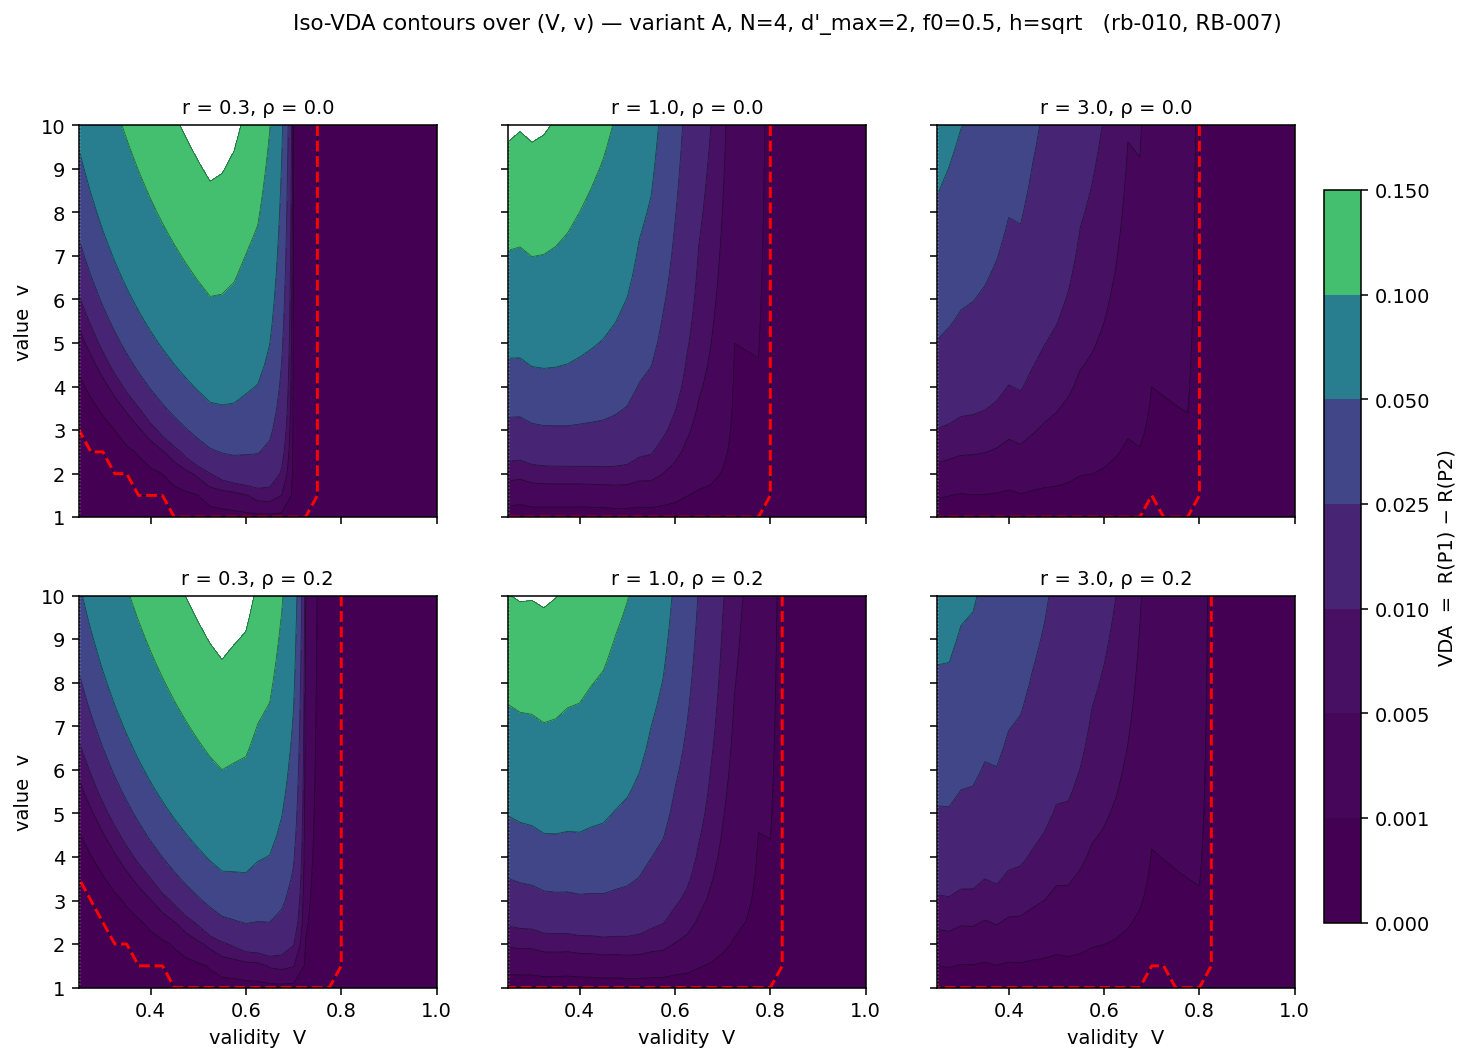
\includegraphics[width=0.98\linewidth]{figures/iso_vda_contours.png}
  \caption{Iso-VDA contour band over the experimental-design plane
  $(\valid, \val)$ at the headline configuration $(\Nloc, \dprimemax,
  f_0, h) = (4,\,2,\,0.5,\,\sqrt{}\,)$, variant~A. Rows: cross-location
  correlation $\corr \in \{0,\, 0.2\}$ (top, independence; bottom, the
  decorrelation channel of Section~\ref{sec:model} at the
  Cohen--Maunsell~\cite{CohenMaunsell2009} cortical anchor $r_{SC}
  \approx 0.2$). Columns: benefit/cost asymmetry $\Rsens \in \{0.3,\,
  1,\, 3\}$. The vertical reference $\valid = 1/\Nloc = 0.25$ is the
  chance baseline; the $\val = 1$ row is the value-blind reference where
  $\VDA \equiv 0$ by construction. Filled contours are at $\VDA \in
  \{0,\,0.001,\,0.005,\,0.01,\,0.025,\,0.05,\,0.1,\,0.15,\,0.2\}$ on a
  common scale. Substantial VDA is confined to a corner along low
  $\valid$ and high $\val$ that flattens as $\Rsens$ rises.}
  \label{fig:iso-vda-contours}
\end{figure}
%
In every panel the bulk of $(\valid, \val)$ space carries near-zero
VDA (median $\VDA \le 0.007$; Table~\ref{tab:graded-marginals}), and
substantial benefit is confined to a corner along low $\valid$ and high
$\val$. The corner flattens along the $\Rsens$-axis: at the
cost-dominant column $\Rsens = 0.3$ it is broad and reaches $\VDA
\approx 0.17$; at the symmetric column $\Rsens = 1$ it narrows to $\VDA
\approx 0.16$; at the benefit-dominant column $\Rsens = 3$ it collapses
to $\VDA \le 0.06$ everywhere on the grid.

\paragraph{Distribution of the benefit across the plane.}
Table~\ref{tab:graded-marginals} summarises the per-panel distribution
of $\VDA$ over the $589 = 31 \times 19$ design cells in each panel.
%
\begin{table}[t]
  \centering
  \small
  \begin{tabular}{c c c c c c c c}
    \toprule
    $\Rsens$ & $\corr$ &
    $\VDA_{\min}$ & median & $q_{95\%}$ & $\VDA_{\max}$ &
    $\mathrm{frac}\!\ge\!0.005$ & $\mathrm{frac}\!\ge\!0.05$ \\
    \midrule
    $0.3$ & $0.0$ & $0$ & $0.0010$ & $0.1289$ & $\mathbf{0.1734}$ & $0.465$ & $0.287$\\
    $0.3$ & $0.2$ & $0$ & $0.0040$ & $0.1328$ & $\mathbf{0.1780}$ & $0.484$ & $0.295$\\
    \midrule
    $1.0$ & $0.0$ & $0$ & $0.0052$ & $0.1152$ & $0.1574$ & $0.503$ & $0.219$\\
    $1.0$ & $0.2$ & $0$ & $0.0069$ & $0.1180$ & $0.1552$ & $0.535$ & $0.236$\\
    \midrule
    $3.0$ & $0.0$ & $0$ & $0.0024$ & $0.0361$ & $0.0619$ & $0.380$ & $0.012$\\
    $3.0$ & $0.2$ & $0$ & $0.0025$ & $0.0390$ & $0.0621$ & $0.402$ & $0.019$\\
    \bottomrule
  \end{tabular}
  \caption{Per-panel distribution of $\VDA$ over the $31 \times 19 =
  589$ $(\valid, \val)$ cells, at the headline configuration $(\Nloc,
  \dprimemax, f_0, h) = (4,\,2,\,0.5,\,\sqrt{}\,)$, variant~A. The
  median $\VDA \le 0.007$ in every panel: most of the design plane
  carries near-zero benefit. The $\mathrm{frac}\!\ge\!0.05$ column
  collapses from $\approx 29\%$ at $\Rsens = 0.3$ to $\le 2\%$ at
  $\Rsens = 3$, quantifying the flattening of the contour band along the
  $\Rsens$-axis.}
  \label{tab:graded-marginals}
\end{table}
%
The peak $\VDA$ over the grid is $0.173$ at $(\Rsens, \corr) = (0.3, 0)$
and falls to $0.062$ at $(3.0, 0)$; the fraction of cells with $\VDA
\ge 0.05$ falls from $28.7\%$ at $\Rsens = 0.3$ to $1.2\%$ at $\Rsens =
3$. At $\corr = 0.2$ this fraction is slightly larger in every panel
($+0.8$ to $+1.7$ percentage points), consistent with the
$\corr$-sensitivity below; the peak and median values are essentially
unchanged in $\corr$ at this magnitude.

\paragraph{A quantitative threshold for spatial cueing designs.}
The contour band yields a concrete design prediction indexed on the
validity threshold. Sweeping $\val \in [1, 10]$ at fixed $\Rsens \in
\{0.3, 1, 3\}$ and $\corr \in \{0, 0.2\}$ at four validity strata
$\valid \in \{0.4, 0.6, 0.8, 0.95\}$, and recording the maximum $\VDA$
in each $(\valid, \Rsens, \corr)$ stratum, gives
Table~\ref{tab:graded-highV}.
%
\begin{table}[t]
  \centering
  \small
  \begin{tabular}{c c c c}
    \toprule
    $\valid$ & $\Rsens = 0.3$ & $\Rsens = 1.0$ & $\Rsens = 3.0$ \\
    \midrule
    $0.40$  & $0.1254\,/\,0.1197$ & $0.1283\,/\,0.1394$ & $0.0329\,/\,0.0391$\\
    $0.60$  & $0.1432\,/\,\mathbf{0.1639}$ & $0.0320\,/\,0.0461$ & $0.0097\,/\,0.0120$\\
    $0.80$  & $0.0000\,/\,0.0000$ & $0.0000\,/\,\mathbf{0.0023}$ & $0.0000\,/\,\mathbf{0.0032}$\\
    $0.95$  & $0.0000\,/\,0.0000$ & $0.0000\,/\,0.0000$ & $0.0000\,/\,0.0000$\\
    \bottomrule
  \end{tabular}
  \caption{Peak $\VDA$ over the $\val$-grid $[1, 10]$ at each $(\valid,
  \Rsens)$ stratum, reported as the pair $\corr = 0\,/\,\corr = 0.2$.
  Entries of $0.0000$ are at the grid floor (no cell on the $\val$-grid
  produced a non-trivial $\VDA$ at the allocation-grid resolution
  $\Delta\alpha = 0.005$). Bold entries flag the threshold transitions
  discussed in the text.}
  \label{tab:graded-highV}
\end{table}
%
The table licenses three statements, each conditional on a quantitative
validity threshold:
\begin{itemize}
  \item \textbf{At $\valid \ge 0.95$}, peak $\VDA$ is at the grid floor
        for every $(\Rsens, \corr)$ in the envelope: a high-validity
        design is predicted to carry negligible VDA at this strict
        threshold.
  \item \textbf{At $\valid \ge 0.80$}, peak $\VDA$ is at the grid floor
        under independence, but admits a small $\corr$-conditional
        signal at $\corr = 0.2$ (maximum $0.0032$ at $\Rsens = 3$).
        ``High validity'' at this threshold therefore carries a
        $\corr$-conditional caveat: under cross-location correlation at
        the Cohen--Maunsell~\cite{CohenMaunsell2009} anchor, a
        sub-percent signal is recoverable in the symmetric and
        benefit-dominant columns.
  \item \textbf{At $\valid \ge 0.60$}, the benefit is substantial: peak
        $\VDA$ reaches $0.1432$ at $(\Rsens, \corr) = (0.3, 0)$ and
        $0.1639$ at $(0.3, 0.2)$. Cost-dominant designs at $\valid \in
        [0.6, 0.8)$ are predicted to carry material VDA, concentrated at
        high cue value.
\end{itemize}
%
The model's experimental-design guidance, anchored to
Table~\ref{tab:graded-highV} and the validity slices of
Figure~\ref{fig:vda-at-high-V}, is therefore:
%
\begin{quote}
  \emph{Spatial cueing paradigms targeting a negligible-VDA regime
  should adopt $\valid \gtrsim 0.95$ unconditionally, or $\valid
  \gtrsim 0.8$ where cross-location correlation can be bounded below
  $r_{SC} \approx 0.2$. A threshold of $\valid \ge 0.75$ is too
  permissive: at $\valid \in [0.6, 0.8)$ the cost-dominant regime
  $\Rsens \in (0, 0.5)$ admits peak $\VDA$ up to $\approx 0.16$, with
  the largest values at high cue value $\val$.}
\end{quote}
%
This guidance is stated at the headline configuration $(\Nloc,
\dprimemax, f_0, h) = (4,\,2,\,0.5,\,\sqrt{}\,)$ under variant~A; the
variant~B and conservation-family bands are taken up in the Discussion
(Section~\ref{sec:discussion}). The validity slices of
Figure~\ref{fig:vda-at-high-V} make the $\val$-axis dependence explicit.
%
\begin{figure}[t]
  \centering
  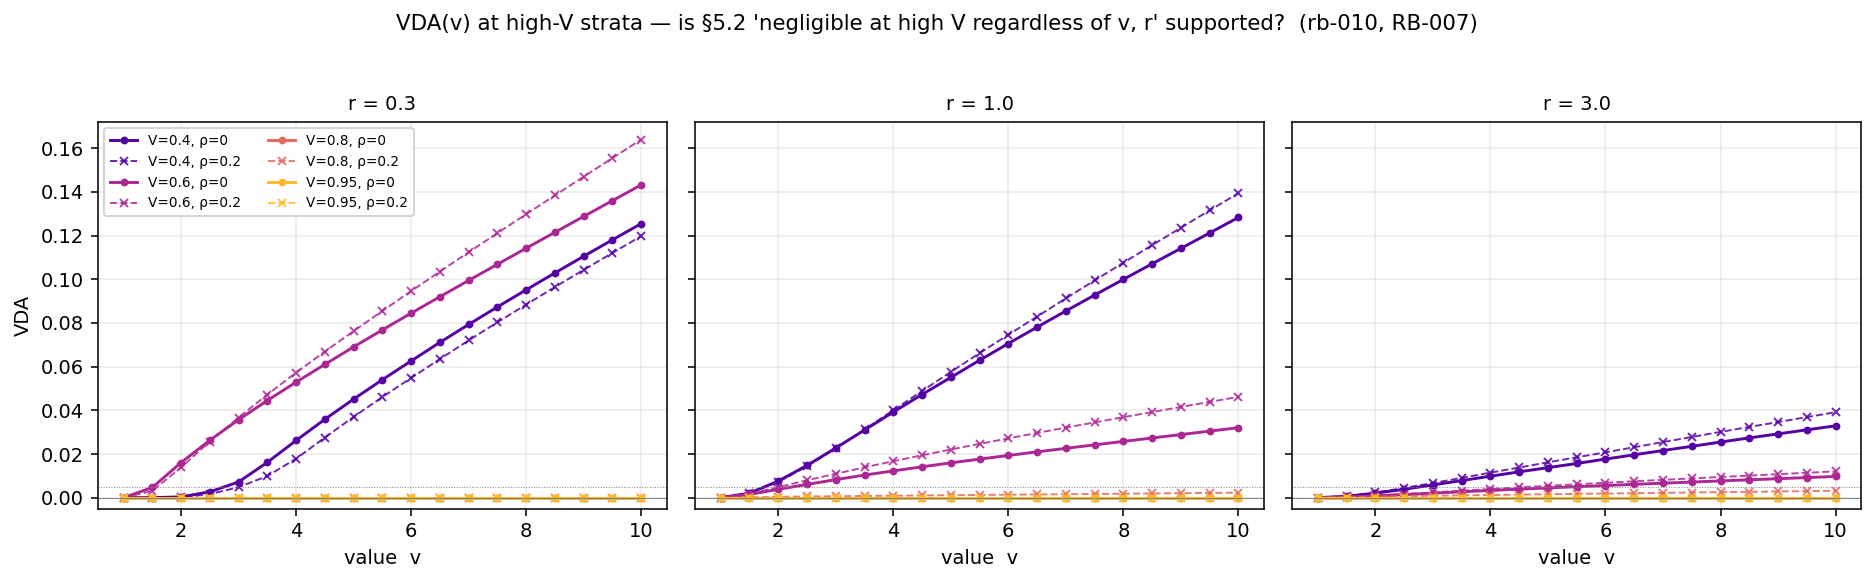
\includegraphics[width=0.95\linewidth]{figures/vda_at_high_V.png}
  \caption{Peak $\VDA(\val)$ at four validity strata $\valid \in
  \{0.4,\,0.6,\,0.8,\,0.95\}$ (curve colour) for each $\Rsens \in
  \{0.3,\,1,\,3\}$ (panel column). Solid: $\corr = 0$; dashed: $\corr =
  0.2$. The $\valid = 0.95$ curve is at the grid floor in every panel;
  the $\valid = 0.80$ curves split between a near-zero $\corr = 0$ line
  and a small $\corr = 0.2$ lift at $\Rsens \in \{1, 3\}$; the $\valid =
  0.60$ curve at $\Rsens = 0.3$ reaches $\VDA = 0.16$ at large $\val$.}
  \label{fig:vda-at-high-V}
\end{figure}

\paragraph{The decorrelation channel reshapes the band.}
The sign of $\partial \VDA / \partial \corr$ is not uniform: across the
design plane, decorrelation amplifies the benefit in some cells and
suppresses it in others. Classifying each $(\valid, \val, \Rsens)$ cell
by the sign of $\Delta\VDA := \VDA(\corr{=}0.2) - \VDA(\corr{=}0)$ gives
the signed contour map of Figure~\ref{fig:iso-vda-drho} and the
per-$\Rsens$ frequencies of Table~\ref{tab:graded-signflip}.
%
\begin{figure}[t]
  \centering
  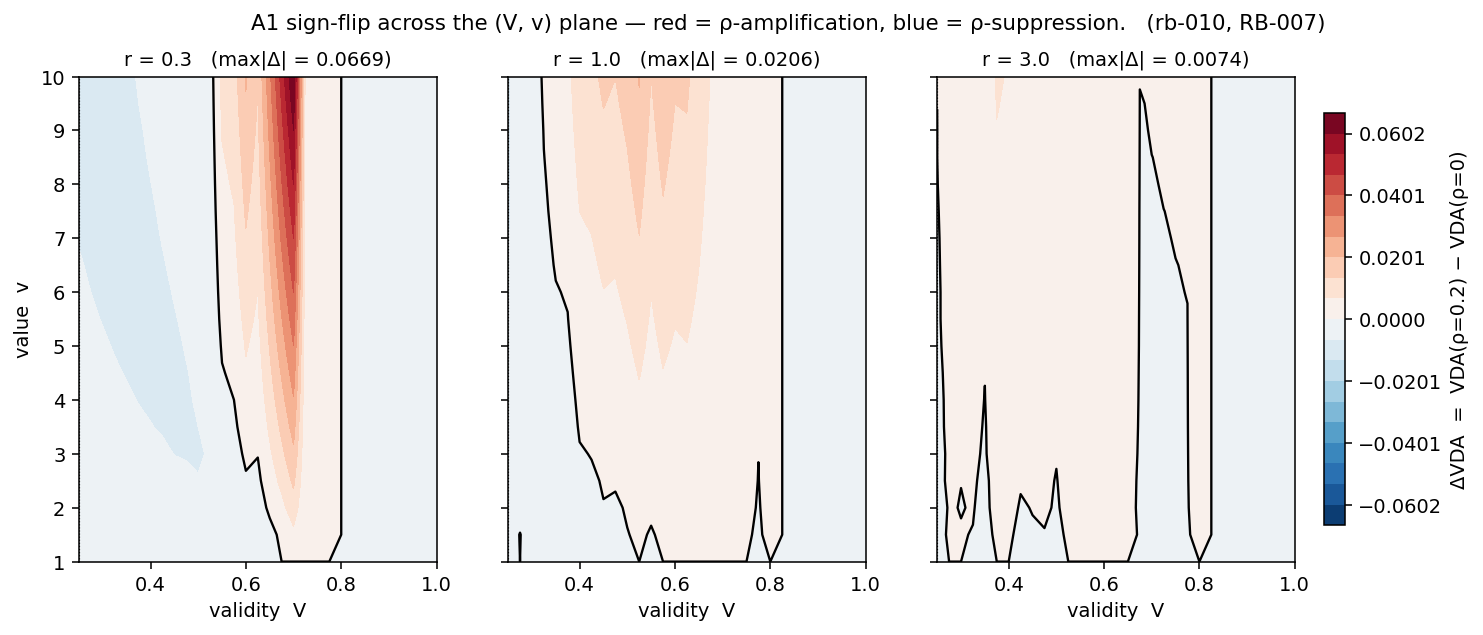
\includegraphics[width=0.95\linewidth]{figures/iso_vda_drho.png}
  \caption{Signed contour map of $\Delta\VDA := \VDA(\corr{=}0.2) -
  \VDA(\corr{=}0)$ over $(\valid, \val)$ for each $\Rsens \in
  \{0.3,\,1,\,3\}$. Red: $\corr$ amplifies $\VDA$; blue: $\corr$
  suppresses; white: $|\Delta\VDA| < 10^{-8}$. At $\Rsens = 0.3$
  (cost-dominant) suppression dominates at low $\valid$; at $\Rsens \in
  \{1, 3\}$ amplification dominates across the bulk of the plane, with
  the strongest amplification near $(\valid, \val) \approx (0.5, 10)$.}
  \label{fig:iso-vda-drho}
\end{figure}
%
\begin{table}[t]
  \centering
  \small
  \begin{tabular}{c c c c c c}
    \toprule
    $\Rsens$ & frac amp & frac supp &
    $\overline{\Delta\VDA}$ & max amp $(\valid, \val)$ & max supp $(\valid, \val)$ \\
    \midrule
    $0.3$ & $27.2\%$ & $\mathbf{37.2\%}$ & $+0.0012$ &
      $+0.0669\;(0.70,\,10)$ & $-0.0105\;(0.25,\,8.5)$\\
    $1.0$ & $\mathbf{52.8\%}$ & $17.5\%$ & $+0.0023$ &
      $+0.0206\;(0.525,\,10)$ & $-0.0084\;(0.25,\,9)$\\
    $3.0$ & $\mathbf{54.0\%}$ & $16.1\%$ & $+0.0009$ &
      $+0.0074\;(0.375,\,10)$ & $-0.0010\;(0.25,\,4.5)$\\
    \bottomrule
  \end{tabular}
  \caption{Cell-wise sign of $\partial \VDA / \partial \corr$ across the
  $(\valid, \val)$ plane at each $\Rsens$ stratum. Fractions are over
  the $589$ cells per panel; the residual share is the zero-class
  $|\Delta\VDA| < 10^{-8}$. Cost-dominant $\Rsens = 0.3$ cells are
  suppression-dominated; the symmetric and benefit-dominant strata are
  amplification-dominated.}
  \label{tab:graded-signflip}
\end{table}
%
Two features stand out. First, the direction of the decorrelation
effect organises along $\Rsens$: cost-dominant cells are suppression-%
dominated, while both the symmetric and benefit-dominant strata are
amplification-dominated, so amplification is not a $\Rsens > 1$
phenomenon but the modal direction once $\Rsens$ exceeds the
$\Rsens \approx 0.4$--$0.6$ sign-flip locus identified in
Section~\ref{sec:results-vda-nonmonotonic}. Second, the largest single
amplification in the entire sweep occurs at $(\valid, \val, \Rsens) =
(0.7,\, 10,\, 0.3)$: a high-validity cell that is essentially dormant
under independence ($\VDA = 0.0007$) lifts to $\VDA = 0.0676$ at $\corr
= 0.2$ --- an $\approx 96\times$ amplification that carries a
normally-negligible design point into the same magnitude as the
low-validity corner. This dormant-cell amplification is a distinctive,
falsifiable consequence of the decorrelation channel, taken up in the
Discussion (Section~\ref{sec:discussion}).

\paragraph{Scope.}
These results are reported at the single configuration $(\Nloc,
\dprimemax, f_0, h) = (4,\,2,\,0.5,\,\sqrt{}\,)$ under variant~A and on
the coarse correlation grid $\corr \in \{0, 0.2\}$. The variant~B and
conservation-family bands are developed in the Discussion
(Section~\ref{sec:discussion}). The validity thresholds are bracketed by
the $\valid$-grid step of $0.025$; a finer grid would sharpen the
``$\gtrsim$'' to a second-decimal number. As an internal consistency
check, the $\val = 1$ column is identically zero across every $(\valid,
\Rsens, \corr)$ cell: the value-blind baseline collapses the joint
optimum onto the value-blind allocation, so $\VDA = 0$ at $\val = 1$ is
a theorem of the model rather than a numerical coincidence.

% Results: optimal allocation does not invert under predictive cues;
% closed-form boundary threshold; anti-cue inversion as a new prediction.
\subsection{Optimal allocation does not invert when the cue is
            predictive}
\label{sec:results-noninversion}

A recurring question in value-cued attention is whether the normative
observer ever does best to attend \emph{away} from the high-value cued
location --- placing less than the uniform share $1/\Nloc$ on it. We
find that under a predictive cue the answer is no: whenever the cued
location carries at least its chance share of the targets, the optimal
allocation $\alphacued^\star$ is at or above $1/\Nloc$ everywhere in the
model's primary operating range. The boundary that governs this fact is
sharp and closed-form, and crossing it --- making the cue
\emph{counter}-predictive --- produces a clean inversion of the optimal
policy that the model predicts quantitatively.

\paragraph{A value-weight inequality sets the no-inversion condition.}
The structural reason no inversion arises is a location-count asymmetry
paired with a value-weight inequality. As $\alphacued \to 1$ the single
cued location reaches its per-location ceiling $\dprime_c = \dprimemax
f(1) = \dprimemax$; as $\alphacued \to 0$ the $\Nloc - 1$ uncued
locations \emph{share} the remaining budget at $(1-\alphacued)/(\Nloc-1)$
each, so each attains only $\dprime_u = \dprime_{\mathrm{base}} +
\benefit(\Rsens)[\dprimemax f(1/(\Nloc-1)) - \dprime_{\mathrm{base}}]
\le \dprimemax$ (strict for $\Nloc \ge 3$, where $f(1/(\Nloc-1)) < 1$).
The per-channel reward weights are $w_c = \valid\,\val$ on the cued slot
and $w_u = (1-\valid)/(\Nloc-1)$ on each uncued slot, and
%
\begin{equation}
  w_c \;\ge\; w_u
  \;\iff\;
  \valid \;\ge\; \frac{1}{(\Nloc - 1)\,\val + 1}.
  \label{eq:value-weight}
\end{equation}
%
For a predictive cue ($\val \ge 1$) the right-hand side of
\eqref{eq:value-weight} is bounded above by $1/\Nloc$, with equality
only at $\val = 1$. The condition $\valid \ge 1/\Nloc$ is therefore the
universal (worst-case-$\val$) sufficient condition for $w_c \ge w_u$,
and the sharp form \eqref{eq:value-weight} carries strictly more slack
as the cued value $\val$ grows. The right branch of the allocation
dominates globally because the larger discriminability sits on the
more-valuable channel.

\paragraph{A closed-form threshold organises the boundary.}
At $\alphacued = 1/\Nloc$ the allocation derivative $\dprime'(\alphacued)$
has a kink, where the benefit/cost roles of $\benefit$ and $\cost$ swap
which side of the linear $\dprime(\alphacued)$ map is active. The
one-sided left derivative of the expected reward at the uniform point
takes the form
%
\begin{equation}
  \left. \frac{\partial \Rpone}{\partial \alphacued} \right|_{1/\Nloc^-}
  \;=\;
  \frac{2\, \dprimemax\, f'(1/\Nloc)}{\Rsens + 1}\,
  \left[
    A_0(\valid, \val, \Nloc, \CR, \corr)
    \;-\;
    \frac{\Rsens}{\Nloc - 1}\, B_0(\valid, \val, \Nloc, \CR, \corr)
  \right],
  \label{eq:boundary-derivative}
\end{equation}
%
where $A_0$ and $B_0$ are the partial derivatives of the expected-reward
functional with respect to $\dprime_c$ and $\dprime_u$ at $\alphacued =
1/\Nloc$, evaluated at the jointly-optimised criteria $(c_c^\star,
c_u^\star)$. Both are $\Rsens$-independent boundary partials --- the
only $\Rsens$-dependence in \eqref{eq:boundary-derivative} sits in the
prefactor and inside the bracket --- so the bracket vanishes at a single
closed-form threshold,
%
\begin{equation}
  \rstarinv(\valid, \val, \Nloc, \CR, \corr)
  \;:=\;
  (\Nloc - 1)\,
  \frac{A_0(\valid, \val, \Nloc, \CR, \corr)}
       {B_0(\valid, \val, \Nloc, \CR, \corr)}.
  \label{eq:r-inv}
\end{equation}
%
For $\Rsens < \rstarinv$ the boundary left derivative is positive (the
uniform point is locally preferred from the left branch); for $\Rsens >
\rstarinv$ it is negative, so the left branch develops a local maximum
at the allocation edge while the global maximum remains on the right
branch at $\alphacued^\star > 1/\Nloc$. The boundary picture above
$\rstarinv$ is thus bimodal, with the value-weight inequality
\eqref{eq:value-weight} deciding which branch is global. The threshold
admits an exact anchor at the symmetric corner $(\valid, \val) =
(1/\Nloc, 1)$, where \eqref{eq:value-weight} holds with equality:
%
\begin{equation}
  \rstarinv(\valid = 1/\Nloc,\, \val = 1,\, \Nloc,\, \CR,\, \corr)
  \;=\; 1
  \qquad \text{exactly,}
  \label{eq:r-inv-corner}
\end{equation}
%
independent of $\Nloc$, the conservation rule $\CR$, and the
correlation $\corr$; the identity is recovered to floating-point
precision at every panel of Table~\ref{tab:noninv-tally}. The full
derivation of \eqref{eq:boundary-derivative}--\eqref{eq:r-inv-corner},
including the corner identity from the joint first-order conditions, is
given in the Supplementary material (Section~\ref{sec:appendix}).

\paragraph{The threshold across the design grid.}
We evaluate \eqref{eq:r-inv} on the primary $(\valid, \val)$ grid
($\valid \in \{0.25, 0.30, \ldots, 1.00\}$, $\val \in \{1, 2, 3, 4,
5\}$) at $\Nloc = 4$ for both reward variants and $\corr \in \{0,
0.2\}$. Per panel we count cells with $\rstarinv \in [0.1, 10]$ (the
asymmetry range over which the boundary derivative sign-flips) versus
$\rstarinv > 10$ (no sign-flip in range; the local picture is
monotone), and report the strict minimum and median
(Table~\ref{tab:noninv-tally}). Aggregated across all $210$ $(\valid,
\val, \text{variant})$ cells at $\corr = 0$, $48.6\%$ have $\rstarinv
\in [0.1, 10]$; under the decorrelation channel at $\corr = 0.2$ the
fraction rises to $51.9\%$ and the median $\rstarinv$ falls by $\sim
13\%$ (variant~A) and $\sim 21\%$ (variant~B), so decorrelation moves
the boundary sign-flip to \emph{smaller} $\Rsens$.
%
\begin{table}[t]
  \centering
  \small
  \begin{tabular}{c c r r r r r}
    \toprule
    variant & $\corr$ & $n$ & $\rstarinv \in [0.1, 10]$ &
    $\rstarinv > 10$ & $\min \rstarinv$ & $\mathrm{median}\,\rstarinv$ \\
    \midrule
    A & $0.0$ & $105$ & $40\,(38.1\%)$ & $65\,(61.9\%)$ &
              $1.0000$ & $17.30$ \\
    A & $0.2$ & $105$ & $42\,(40.0\%)$ & $63\,(60.0\%)$ &
              $1.0000$ & $15.08$ \\
    B & $0.0$ & $105$ & $62\,(59.0\%)$ & $43\,(41.0\%)$ &
              $1.0000$ & $\phantom{0}7.64$ \\
    B & $0.2$ & $105$ & $68\,(64.8\%)$ & $37\,(35.2\%)$ &
              $1.0000$ & $\phantom{0}6.02$ \\
    \bottomrule
  \end{tabular}
  \caption{Closed-form inversion threshold $\rstarinv$ from
  \eqref{eq:r-inv} on the primary $(\valid, \val)$ grid at $\Nloc = 4$,
  by reward variant and correlation $\corr$. The $\rstarinv =
  1.0000$ minimum in every panel is the symmetric-corner identity
  \eqref{eq:r-inv-corner}. Variant~B admits the local sign-flip across
  roughly twice as many cells as variant~A; the decorrelation channel
  ($\corr = 0.2$) shifts the sign-flip to smaller $\Rsens$, lowering the
  median threshold in both variants.}
  \label{tab:noninv-tally}
\end{table}
%
The contour structure of $\rstarinv(\valid, \val)$ at $\corr = 0$ is
shown in Figure~\ref{fig:r-inv-map}. The $\rstarinv = 1$ contour passes
through the symmetric corner in both variants, consistent with
\eqref{eq:r-inv-corner}, and the $\rstarinv = 10$ contour bounds the
region in which the uniform point stays locally stable across the entire
$\Rsens \in [0.1, 10]$ range.
%
\begin{figure}[t]
  \centering
  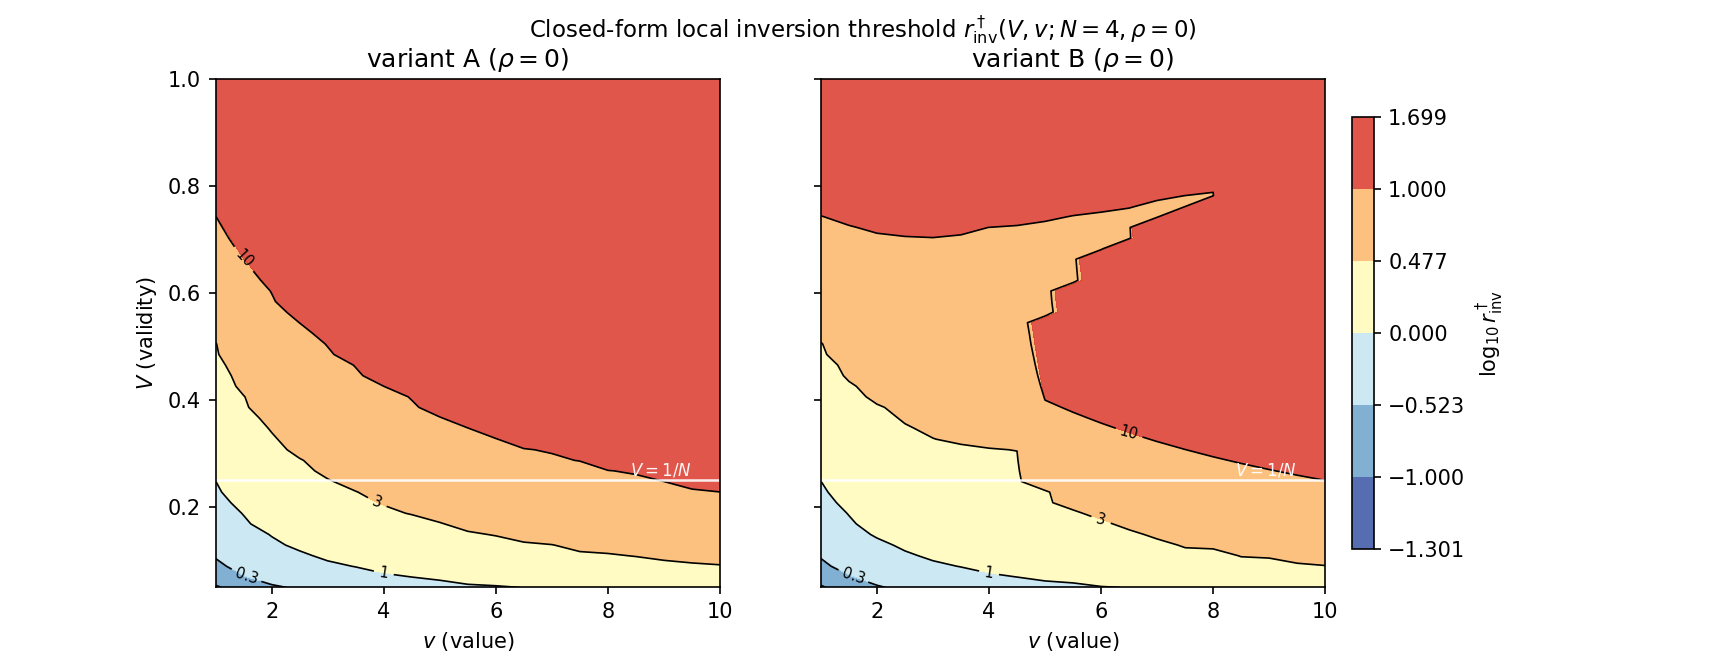
\includegraphics[width=0.95\linewidth]{figures/r_inv_closed_form.png}
  \caption{Contour map of $\log_{10}\rstarinv(\valid, \val)$ at $\Nloc =
  4$, $\corr = 0$, for reward variant~A (left) and variant~B
  (right), evaluated from \eqref{eq:r-inv}--\eqref{eq:r-inv-corner}.
  Black contours at $\rstarinv \in \{0.1, 0.3, 1, 3, 10\}$. The
  $\rstarinv = 1$ contour passes through the symmetric corner $(\valid,
  \val) = (0.25, 1)$ in both panels (the identity
  \eqref{eq:r-inv-corner}); the $\rstarinv = 10$ contour bounds the
  region with no boundary sign-flip inside $\Rsens \in [0.1, 10]$.
  Variant~B admits the sign-flip across more cells than variant~A
  ($59.0\%$ vs.\ $38.1\%$; Table~\ref{tab:noninv-tally}).}
  \label{fig:r-inv-map}
\end{figure}

\paragraph{No global inversion across the predictive-cue sweep.}
The local sign-flip of \eqref{eq:boundary-derivative} does not by itself
produce a global inversion: even where $\Rsens > \rstarinv$ and the
bracket is negative, the left-branch local maximum sits at the
allocation edge while the right-branch global maximum sits at
$\alphacued^\star > 1/\Nloc$, by the location-count argument above. We
confirm this directly by sweeping $\Rew(\alphacued)$ on the full
allocation grid $[0.02, 1.0]$ at step $0.005$ for the most adversarial
primary-sweep cells (those with the smallest $\rstarinv$ at $\Rsens =
10$, most likely to favour the left branch), at both $\corr \in \{0,
0.2\}$. Across all $12$ probes the result is uniform:
$\alphacued^\star \ge 1/\Nloc$, and the right-branch global maximum
strictly dominates (Table~\ref{tab:noninv-sweep}). The no-inversion
property holds at $\corr = 0$ and is unchanged under the decorrelation
channel at $\corr = 0.2$.
%
\begin{table}[t]
  \centering
  \small
  \begin{tabular}{c r c c r r r r}
    \toprule
    $\valid$ & $\val$ & variant & $\corr$ &
    $\rstarinv$ & $\alphacued^\star$ &
    $\Rew_{\mathrm{global}}$ & $\Rew_{\mathrm{left}}$ \\
    \midrule
    $0.250$  & $1$ & A & $0.0$ & $1.0000$    & $0.955$ &
    $0.65936$ & $0.64564$ \\
    $0.250$  & $1$ & A & $0.2$ & $1.0000$    & $0.950$ &
    $0.66809$ & $0.65550$ \\
    $0.250$  & $1$ & B & $0.0$ & $1.0000$    & $0.955$ &
    $0.65936$ & $0.64564$ \\
    $0.250$  & $1$ & B & $0.2$ & $1.0000$    & $0.950$ &
    $0.66809$ & $0.65550$ \\
    $0.2875$ & $1$ & A & $0.0$ & $1.2483$    & $0.970$ &
    $0.66541$ & $0.64462$ \\
    $0.325$  & $1$ & A & $0.2$ & $\sim\!1.6$ & $0.975$ &
    $0.67997$ & --- \\
    \bottomrule
  \end{tabular}
  \caption{Six representative full-allocation probes from the $12$-probe
  sweep at $\Rsens = 10$ at the most adversarial predictive-cue cells.
  In every probe $\alphacued^\star \ge 1/\Nloc = 0.25$, with the
  right-branch global maximum at $\alphacued^\star \in [0.95, 0.98]$
  strictly dominating the left-branch local maximum (at the grid edge
  $\alphacued = 0.02$). Across all $12$ probes the number of global
  inversions is $\mathbf{0}$, at both $\corr = 0$ and $\corr = 0.2$.}
  \label{tab:noninv-sweep}
\end{table}
%
The boundary geometry is illustrated in
Figure~\ref{fig:er-alpha-anticue}, which plots $\Rew(\alphacued)$ for a
family of asymmetry ratios. The kink at $\alphacued = 1/\Nloc$ becomes a
local minimum once $\Rsens > \rstarinv$, with local maxima on both
branches; which branch wins globally is set by the value-weight
inequality \eqref{eq:value-weight}. The panel is drawn at a
counter-predictive cell $(\valid, \val) = (0.15, 1)$, where
\eqref{eq:value-weight} fails, so the reader sees both regimes of the
boundary at once --- the subject of the next paragraph.
%
\begin{figure}[t]
  \centering
  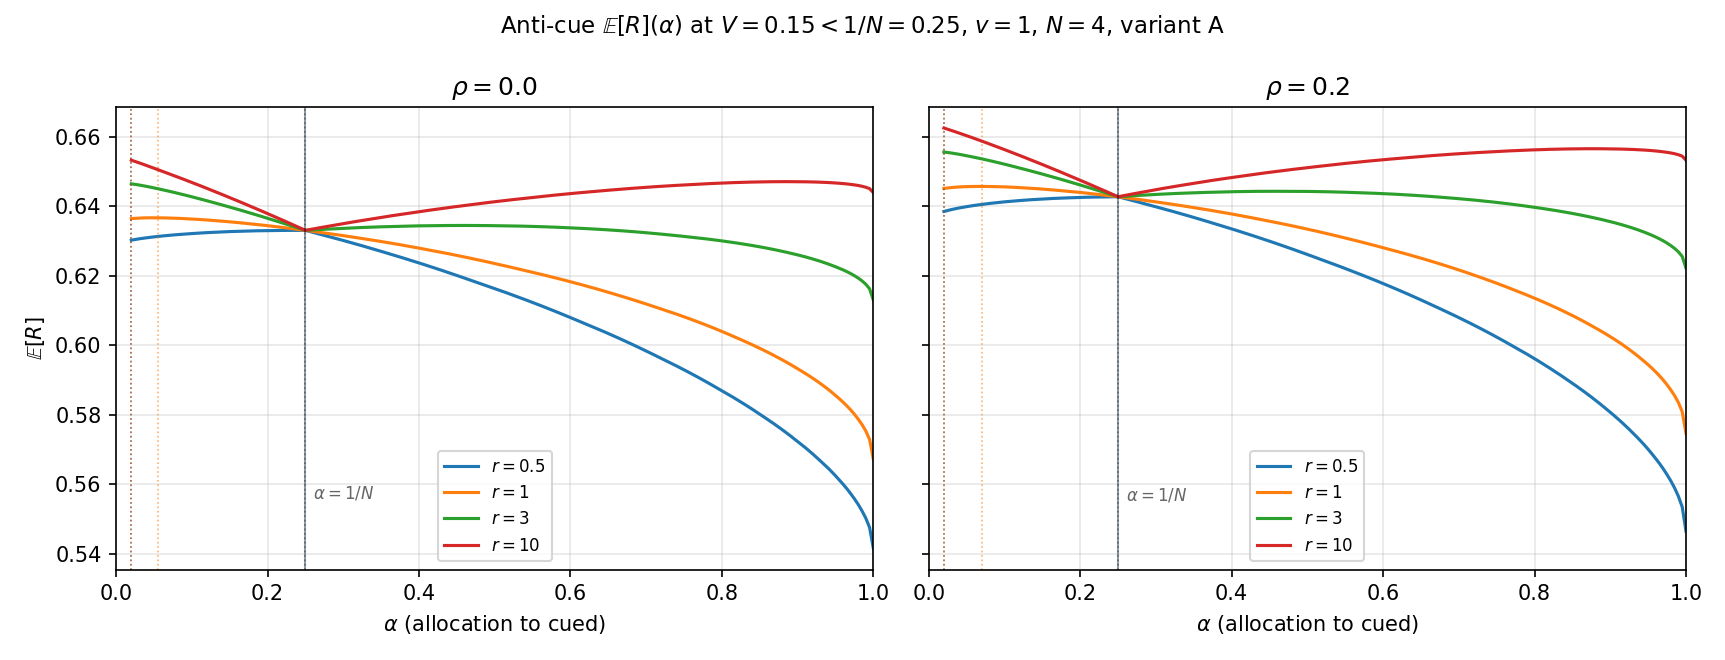
\includegraphics[width=0.95\linewidth]{figures/er_vs_alpha_anticue.png}
  \caption{Expected reward $\Rew(\alphacued)$ on the full allocation
  grid at the counter-predictive cell $(\valid, \val, \Nloc) = (0.15, 1,
  4)$ for $\Rsens \in \{0.5, 1, 3, 10\}$, at $\corr = 0$ (left) and
  $\corr = 0.2$ (right). The kink at $\alphacued = 1/\Nloc = 0.25$ is
  the benefit/cost swap of the allocation map; for $\Rsens > \rstarinv$
  it is a local minimum, with both branches admitting local maxima.
  Because $\valid < 1/\Nloc$ here, the value-weight inequality
  \eqref{eq:value-weight} fails and the left-branch maximum (at the grid
  edge $\alphacued = 0.02$) dominates globally for $\Rsens \ge 1$ --- the
  counter-predictive inversion. The decorrelation channel at $\corr =
  0.2$ leaves the bimodality and the inversion onset unchanged.}
  \label{fig:er-alpha-anticue}
\end{figure}

\paragraph{Counter-predictive cues invert the optimal policy.}
The model makes a clean prediction once the cue is counter-predictive.
At $\valid < 1/\Nloc$ (sharply, $\valid < 1/[(\Nloc-1)\val + 1]$) the
value-weight inequality \eqref{eq:value-weight} flips, $w_c < w_u$, and
the location-count argument runs in reverse: the larger discriminability
would sit on the less-valuable channel, so the global optimum drops to
$\alphacued^\star < 1/\Nloc$ and the normative observer attends
\emph{away} from the low-validity location toward the population of
alternatives. We probe a counter-predictive sub-grid $\valid \in \{0.05,
0.10, 0.15, 0.20\}$ (all below $1/\Nloc = 0.25$), $\val \in \{1, 3, 5\}$,
$\Rsens \in \{0.1, 0.5, 1, 3, 5, 10\}$, variant~A, at $\corr \in \{0,
0.2\}$. The global-inversion incidence is $26/72 = 36.1\%$ at $\corr =
0$ and $25/72 = 34.7\%$ at $\corr = 0.2$, and it stratifies cleanly
along the sharp boundary \eqref{eq:value-weight}
(Table~\ref{tab:anticue}).
%
\begin{table}[t]
  \centering
  \small
  \begin{tabular}{l r r r r r r}
    \toprule
    & \multicolumn{6}{c}{Inversion incidence at $\corr = 0$
      (values $\to$ inversions / total)} \\
    \midrule
    by $\Rsens$ &
    $\Rsens{=}0.1{:}\ 1/12$ &
    $\Rsens{=}0.5{:}\ 3/12$ &
    $\Rsens{=}1{:}\ 6/12$ &
    $\Rsens{=}3{:}\ 6/12$ &
    $\Rsens{=}5{:}\ 6/12$ &
    $\Rsens{=}10{:}\ 4/12$ \\
    by $\val$ &
    $\val{=}1{:}\ 18/24$ &
    $\val{=}3{:}\ 5/24$ &
    $\val{=}5{:}\ 3/24$ &
     & & \\
    by $\valid$ &
    $\valid{=}0.05{:}\ 14/18$ &
    $\valid{=}0.10{:}\ 5/18$ &
    $\valid{=}0.15{:}\ 4/18$ &
    $\valid{=}0.20{:}\ 3/18$ &
    & \\
    \bottomrule
  \end{tabular}
  \caption{Counter-predictive inversion incidence
  ($\alphacued^\star < 1/\Nloc$) at $\Nloc = 4$, variant~A, $\corr = 0$,
  stratified by $\Rsens$, $\val$, and $\valid$ (total $26/72 = 36.1\%$).
  Incidence rises from $8.3\%$ at $\Rsens = 0.1$ to $50\%$ at $\Rsens
  \in \{1, 3, 5\}$ and tapers to $33.3\%$ at $\Rsens = 10$, where the
  strong-asymmetry regime begins to re-favour the right branch. The
  value dependence is the key qualitative signature predicted by
  \eqref{eq:value-weight}: inversion is dense at $\val = 1$ ($75\%$) but
  rare at $\val = 5$ ($12.5\%$), because at $\val = 5$ the inversion
  boundary shrinks to $\valid < 1/[(\Nloc-1)\val + 1] = 1/16 = 0.0625$,
  confining inversion to the $\valid = 0.05$ row. Under the
  decorrelation channel ($\corr = 0.2$) total incidence is $34.7\%$,
  within one cell of $\corr = 0$ across every stratifier.}
  \label{tab:anticue}
\end{table}
%
Figure~\ref{fig:alpha-star-map} maps $\alphacued^\star(\valid, \Rsens)$
at fixed $\val = 5$. The inversion region lies entirely below $\valid =
0.05$, matching the sharp boundary $\valid < 1/16 \approx 0.0625$, and
there are \emph{zero} inversions in the predictive-cue regime $\valid
\ge 1/\Nloc$ at either correlation. The no-inversion property is thus a
conditional theorem --- it holds whenever the cue is predictive --- and
the counter-predictive inversion is a falsifiable prediction the model
makes outside that regime.
%
\begin{figure}[t]
  \centering
  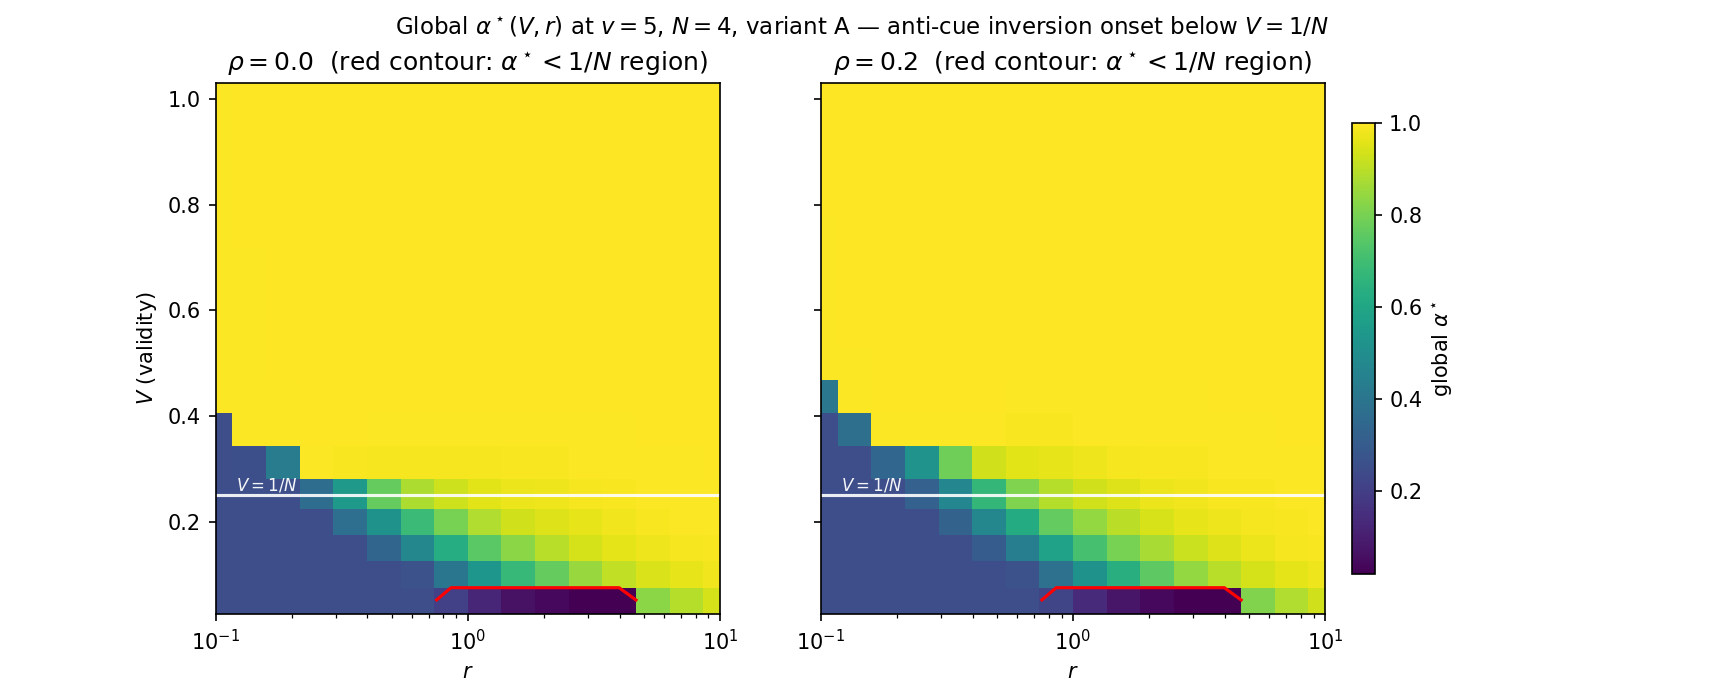
\includegraphics[width=0.95\linewidth]{figures/alpha_star_V_r_map.png}
  \caption{Optimal allocation $\alphacued^\star(\valid, \Rsens)$ at
  $(\Nloc, \dprimemax, f_0, h, \val) = (4,\,2,\,0.5,\,\sqrt{}\,,5)$,
  variant~A, for $\corr = 0$ (left) and $\corr = 0.2$ (right); heat
  scale $\alphacued^\star \in [0.02, 1.0]$. The white horizontal line
  marks the validity threshold $\valid = 1/\Nloc = 0.25$; the red
  contour bounds the inversion region $\alphacued^\star < 1/\Nloc$. The
  inversion region is confined to $\valid \le 0.05$ (consistent with the
  sharp boundary $\valid < 1/16 \approx 0.0625$ from
  \eqref{eq:value-weight}); inversion incidence is $6/272 = 2.21\%$ in
  both panels, with \emph{zero} inversions in the predictive-cue regime
  $\valid \ge 1/\Nloc$.}
  \label{fig:alpha-star-map}
\end{figure}

\paragraph{Robustness and decorrelation sensitivity.}
The no-inversion result is robust across the model's parameters. The
empirical sweep finds $\alphacued^\star \ge 1/\Nloc$ at every cell of
the predictive-cue range under both reward variants, and the
decorrelation channel does not abolish the picture: at $\corr = 0.2$ the
median threshold $\rstarinv$ shifts by $13$--$21\%$, the predictive-cue
sweep still returns $0$ inversions, and the counter-predictive incidence
moves by at most one cell ($25$ vs.\ $26$ inversions). Decorrelation and
the inversion lever are therefore independent: $\corr$ moves \emph{where}
on the $\Rsens$-axis the boundary derivative sign-flips, but it does not
flip the value-weight inequality \eqref{eq:value-weight} that decides
which branch is globally optimal, so the conditional theorem and its
counter-predictive complement hold at both correlation values.

\paragraph{Relation to the behavioural record.}
The conditional picture aligns with the behavioural literature on
spatial value and statistical learning. When a location holds a target
with below-chance probability, observers learn to suppress it: capture
and target-selection efficiency at the location fall
\cite{wang_theeuwes2018_statistical_learning_distractor_suppression},
fewer saccades land there and latencies to targets there rise
\cite{wang_samara_theeuwes2019}, and selection is reallocated toward the
alternatives \cite{kong_li_wang_theeuwes2020}. In the model's
coordinates a below-chance location has validity $\valid < 1/\Nloc$ ---
exactly the regime in which \eqref{eq:value-weight} predicts inversion
--- so the behavioural pattern is a prediction match: the normative
observer should allocate below uniform there, and observers do.
Conversely, in the predictive-cue regime $\valid \ge 1/\Nloc$ the model
says the observer should never go below uniform, and the
value-driven-capture literature reports the opposite mistake, observers
pulled \emph{toward} high-value locations even when maladaptive
\cite{failing_theeuwes2018_selection_history,
hickey2010_reward_salience_acc}, consistent with the no-inversion
direction. The chance-validity case $\valid = 1/\Nloc$
\cite{posner1980_orienting} sits at the boundary, where the model
collapses to a tied optimum and no reallocation is predicted.

\paragraph{Scope.}
The counter-predictive sweep is reported for variant~A; the lower median
$\rstarinv$ of variant~B (Table~\ref{tab:noninv-tally}) indicates a
somewhat higher inversion incidence there, mapped in the Discussion
(Section~\ref{sec:discussion}). The validity grid is at step $0.05$, so
the inversion-onset validity between $\valid = 0.20$ and the boundary
$\valid = 0.25$ at $\val = 1$ is bracketed to $\pm 0.05$; a finer grid
would localise it. As a consistency check, the symmetric corner
$(\valid, \val) = (1/\Nloc, 1)$ returns $\rstarinv = 1$ to
floating-point precision across all variants and correlations
\eqref{eq:r-inv-corner}, and at $\val = 1$ the model is value-blind so
the predictive and counter-predictive regimes meet at a tied optimum.
